\documentclass[11pt]{article}

% --- Packages ---
\usepackage[utf8]{inputenc}
\usepackage{amsmath, amssymb, amsthm}
\usepackage{graphicx}
\usepackage{enumitem}
\usepackage[margin=1in]{geometry} 
\usepackage{colortbl} 
\usepackage{array}    
\usepackage{titlesec}
\usepackage{enumitem}
\usepackage{xcolor}
\usepackage[most]{tcolorbox}
\usepackage{listings}
\usepackage{booktabs}
\usepackage{siunitx}
\usepackage{parskip}
\usepackage{float}
\usepackage{caption}
\usepackage{xcolor}
\usepackage{listings}
\usepackage{tabularx}
\usepackage{amssymb}
\usepackage{tikz}
\usepackage{pgfplots}
\pgfplotsset{compat=1.18}
\usepackage{hyperref}
\usepackage{pgfplots}
\usepackage{multicol}   

\pgfplotsset{compat=1.18}

\sisetup{
  group-separator={,},
  group-minimum-digits=4,
  round-mode=places,
  round-precision=2,
  input-ignore={,} % <-- allows commas in input
}

\setlength{\parskip}{6pt}

\setcounter{secnumdepth}{0}

\definecolor{darkblue}{rgb}{0,0,0.8}

\hypersetup{
  colorlinks=true,
  linkcolor=darkblue,
  citecolor=darkblue,
  urlcolor=darkblue
}


\setlist[itemize]{label=--}

\lstset{
  language=Python,
  basicstyle=\ttfamily\small,
  keywordstyle=\color{blue}\bfseries,
  commentstyle=\color{gray},
  stringstyle=\color{orange},
  showstringspaces=false,
  numbers=left,
  numberstyle=\tiny\color{gray},
  breaklines=true,
  frame=single,
  captionpos=b
}

% --- Theorem Environments ---
\theoremstyle{definition}
\newtheorem{definition}{Definition}[section]
\newtheorem{example}{Example}[section]

\theoremstyle{plain}
\newtheorem{theorem}{Theorem}[section]
\newtheorem{lemma}[theorem]{Lemma}

% --- Custom Commands ---
\newcommand{\R}{\mathbb{R}}
\newcommand{\E}{\mathbb{E}}
\newcommand{\Var}{\mathrm{Var}}
\newcommand{\Cov}{\mathrm{Cov}}
\newcommand{\prob}[1]{\mathbb{P}\left(#1\right\)}
\newcommand{\norm}[1]{\left\lVert#1\right\rVert}

\newcommand{\altrowtable}[3]{%
  \renewcommand{\arraystretch}{1.4} 
  \begin{minipage}{0.95\linewidth}
  \rowcolors{1}{gray!10}{white}
  \begin{tabular}{@{} >{\raggedright\arraybackslash}m{#1\linewidth} m{#2\linewidth} @{}}
  #3
  \end{tabular}
  \end{minipage}
}

\lstdefinestyle{rstyle}{
    language=R,
    basicstyle=\ttfamily\footnotesize,
    keywordstyle=\color{blue},
    commentstyle=\color{gray},
    stringstyle=\color{red},
    showstringspaces=false,
    breaklines=true
}

% Box style
\tcbset{
  qa/.style={
    colback=white,
    colframe=black,
    coltitle=black,
    fonttitle=\small\bfseries,
    fontupper=\small,   % �� makes content smaller
    sharp corners,
    boxrule=0.3pt,
    enhanced,
    breakable,
    colbacktitle=white
  }
}

\titlespacing*{\section}{0pt}{*1}{*0.5}
\titlespacing*{\subsection}{0pt}{*0.5}{*0.25}
\setlist{noitemsep, topsep=0pt}

% --- Document Start ---
\begin{document}

% --- Title Page ---
\begin{titlepage}
    \centering
    \vspace*{3cm}
    {\Huge\bfseries STA 280: Unsupervised Learning \par}
    \vspace{1.5cm}
    {\Large Gabriel Kinshuk \par}
    \vfill
    {\large Spring 2026 \par}
\end{titlepage}

% --- Table of Contents ---
\tableofcontents
\clearpage

\newpage

\section{Introduction}

\bigskip

\subsection{Grading Policies}

\medskip

Grades are based on a 1000 point scale, with no predetermined cutoff for letter grades:
\begin{itemize}
    \item Final Exam - 500 points
    \item Homework - 200 points
    \item Quizzes - 200 points
    \item Participation - 100 points
\end{itemize}

\medskip

There will be homework every week, which can collaborate on with \textit{one} other student. Every class begins with a 10-point quiz, which are closed book and have two drops. Homework and quiz points may not exactly add up to 200 but will be adjusted to a 200 point scale. 

The final exam will be on February 28.


\bigskip

\subsection{Machine \& Statistical Learning}

\medskip

Learning from data is called both \textit{machine learning} and \textit{statistical learning}. In machine learning the goal is often prediction, while in statistical learning the goal is often inference. 

In unsupervised learning there is no way to predict a dependent $Y$ from independent variables $X$ (no training data set). Instead, we are attempting to understand the structure of $X$. 

We may have a data matrix $X_{n\times p}$ with $n$ observations and $p$ features. Our goal is to discover the row and column structure of $X$. Two methodology classes include cluster analysis and dimensionality reduction:

\begin{itemize}
    \item Cluster analysis: simplify $X$ by clustering into similar rows/observations
    \item Dimensionality reduction: simplify $X$ by combining columns into new variables
\end{itemize}


\section{Cluster Analysis}

\medskip

Cluster analysis (CA) uncovers structure in a dataset by aggregating similar rows into groups called clusters. Contrasting with PCA which reduces the number of columns, CA does not actually reduce the number of rows. Grouping can be based on measures of similarity \textit{or} dissimilarity among the rows. The two major problems are determining the number of clusters and how to assign rows to clusters. 

We can view classification problems as supervised clustering, where the number of clusters (classes) is known and we have a training set of rows that is already correctly classified from which to learn classification rules from. 

When calculating similarity between rows to be clustered, we often consider two quantities: correlation and distance. Correlation has a few issues, some of which include confusing units or questions of how to weight variables (or assume all variables have equal weight as in standardization). Distance measures are much more common to use. 

When treating a cluster as a single entity for interpretation, we typically use the cluster's centroid and member counts of each cluster.

We identify five ways to cluster:
\begin{enumerate}
    \item Single linkage (nearest neighbor)
    \item Complete linkage (farthest neighbor)
    \item Average linkage (average neighbor)
    \item Centroid method
    \item Ward's method
\end{enumerate}

Of which Ward's method is the default for the R package \texttt{hclust}. Ward's method attempts to minimize the within-cluster sum of squares:
\[
\sum_{k=1}^p \sum_{i=1}^c \sum_{l=1}^{n_i} (X_{ikl} - \overline{X}_{ik})^2
\]

\medskip

The total sum of squares, that is the variability of the data, can be written as the sum of the (weighted) deviations of the cluster means from the grand mean (between-cluster sum of squares) plus the deviations of the data from the cluster means (within-cluster sum of squares):
\[
TSS = BSS + WSS
\]

Once we have a given dataset of size $n$, the TSS is fixed. At the maximum number of clusters, $n$, the BSS equals the TSS and WSS is zero. As we decrease the number of clusters, the BSS decreases and the WSS increases until the BSS is zero and the WSS equals the TSS (at one cluster).

We can measure how much of the $X$ variables can be explained by the clustering of the cases by regressing the $X$'s on the clustering. This $R^2$ turns out to be equal to $\frac{BSS}{TSS}$. Then, BSS is the sum of square for the regression, and WSS is the sum of squares for the \textit{error}. 

As a note, the regression of the $X$'s on cluster indicator variables is equivalent to ANOVA, analysis of variance (or when done over multiple $p$ response variables, MANOVA). 

\bigskip


\subsection{K-means CA}

\medskip

Some key R commands are: \texttt{kmeans, pairs, plot3d, scale, set.seed}.

With \texttt{kmeans} sub-objects: \texttt{\$cluster, \$centers, \$tot.withinss, \$betweenss, \$size}.

\medskip

$K$-means cluster analysis works by \textit{iterative partitioning} (IP). IP begins by choosing a set of $K$ initial cluster seeds, often choosing actual cases (observations) themselves as the initial seeds. At each generation, each cluster produces a seed for the next generation, often the centroid (mean vector) is chosen. 

In K-means clustering, for each generation each case is reassigned to the nearest centroid. The seeds are then recalculated and points are reassigned, in a cycle. The cycle continues until either: Data points are no longer reassigned to different clusters or we reach some pre-specified limit of number of passes. K-means is sensitive to the initial partition, and a poor initial seed can lead to poor performance. To deal with this, the clustering is often performed multiple times with different initial seeds. Additionally, we typically repeat this entire process for multiple values of $K$.

\bigskip

\subsection{Hierarchical Agglomerative Clustering}

\medskip

Some key R commands are: \texttt{hclust, cutree, scale, rect.hclust, aggregate} and the \texttt{hclust} sub-object \texttt{\$height}.

Ward's method works hierarchically (clusters organized into tree with parent-child relationships) and agglomeratively (bottom-up, individal data points merge into larger clusters). In contrast, K-means works iteratively, repeatedly reassigning points to find the best fit. 

\medskip

    \begin{table}[H]
\centering
\renewcommand{\arraystretch}{1.5}
\rowcolors{2}{gray!10}{white}
\begin{tabularx}{0.9\textwidth}{l X X}
\toprule
\textit{Feature} 
& \textit{Ward's Method} 
& \textit{K-means Clustering} \\
\midrule
Mathematical objective 
& Minimize within-cluster sum of squares (WSS) 
& Minimize within-cluster sum of squares (WSS) \\

Operational logic 
& Hierarchical and agglomerative 
& Iterative refinement \\

Cluster count 
& Produces solutions for all possible numbers of clusters 
& Produces a solution for a single specified number ($k$) \\

Starting point 
& Starts with $n$ singleton clusters (bottom-up) 
& Starts with $k$ initial centroids \\

Process 
& Successively merges closest pairs of clusters 
& Repeatedly reassigns cases to the nearest centroid \\

Flexibility 
& Membership is fixed once clusters are merged 
& Membership changes until convergence \\
\bottomrule
\end{tabularx}
\caption*{Comparison of Ward's Method and K-means Clustering}
\end{table}

\medskip

As with any model, we need to balance explanatory power with interpretability. We have a few choices for when to end the agglomeration:
\begin{itemize}
    \item Visually: examine the dendrogram and cut the tree as close to the leaves (terminal nodes) without creating too many branches
    \item Quantitatively: we choose a hierarchy level ($k$) as close to the end as possible that still retains a high $R^2$. 
\end{itemize}

\bigskip

\subsection{Cluster Model Selection}

\medskip

Some key R commands are:
\begin{itemize}
    \item \texttt{fviz\_cluster}: plots PC2 vs PC1 for a proposed $k$
    \item \texttt{fviz\_nbclust}: scree plot for Elbow method
    \item \texttt{clusGap}: computes Gap statistic for range of $k$’s
    \item \texttt{fviz\_gap\_stat}: plots Gap statistic for range of $k$’s
\end{itemize}

\medskip

There are a few heuristics for choosing the number of clusters as well as the clustering method:
\begin{enumerate}
    \setlength{\itemsep}{1em}
    \item Domain knowledge: if there is some conventional wisdom for your field about a "natural" number of clusters then it should be included in the set of possible $k$'s to try. 
    \item Elbow method: similar to a scree plot. Plot WSS by number of clusters, if an "elbow" exists then choose the $k$ immediately preceding the plateau. Note that this method is subjective and there may in fact be no elbow.
    \begin{itemize}[label=--]
        \item WSS(k) is the variability of the clustering variables that is unexplained by the k clusters, and BSS(k) is the explained variability
        \item Therefore the plot of WWS($k$) by $k$ shows how unexplained variance decreases with complexity
    \end{itemize}
    \item For any promising $k$, also try values nearby such as $k\pm 1, k\pm 2$ and distinguish them based on differences in $R^2$, AIC (Akaike Information Criterion), or BIC (Bayesian Information Criterion).
    \item Cubic clustering criterion (CCC). Possible $k$'s will be local peaks in the plot of CCC against number of clusters. The CCC evaluates the optimal number of clusters by comparing the observed $R^2$ of a dataset against the expected $R^2$ under the null hypothesis that the data follows a random uniform distribution within the volume of the feature space.
    \item Hierarchical methods do not need to pre-specify a $k$. Further, since we produce a complete genealogy, every cluster for one $k$ is related to every other $k$. If the relationship between $k$'s does not matter, then $K$-means may be appropriate.
    \item We can examine the \textit{silhouette}, which is a measure of how similar a case is to the other cases in its own cluster, relative to how dissimilar the case is to cases in all other clusters. The average silhouette for a clustering $k$ is the mean of the silhouette of all cases. We can then plot the average silhouette against the number of clusters, and we can choose the $k$ with the maximum average silhouette. 
    \item The Gap Statistic Method. This suggests the $k$ that tries to maximize the gap between the expected value of WSS(k) if there were no clusters and the observed value of WSS(k). This requires us to define a \textit{reference distribution} which is uniform along each variable (similar to the assumption in CCC). We then take $B$ samples from the reference distribution and cluster on them with each candidate $k$. For each sample $B$ with $k$ clusters we will then get a WSS, which we take the log of and save for later. The averages of all of the resultant log(WSS) are saved and used as the expected WSS for the gap calculation. Then, we find the observed WSS(k) for our actual dataset and log that as well. We finally choose the the $k$ with the greatest gap.
\end{enumerate}

\subsubsection{Silhouette}

To find the silhouette for a single case, we first calculate two quantities, $a_i$ and $b_i$. $a_i$ is mean distance of case i to all other cases in its cluster, and $b_i$ is the mean distance to all cases in the \textit{next best} cluster (i.e., the cluster that the point would be reassigned to if it \textit{must} be reassigned). We then take the difference between the two and scale it by the larger of the quantities:
\[
s_i = \frac{b_i - a_i}{\max(a_i, b_i)}
\]
So, the silhouette score evaluates if a point is a strong member of its current group or if it is a ``borderline case" that could just as easily belong elsewhere. The average silhouette is the mean silhouette of all cases $i$ in the dataset. A larger average silhouette indicates a stronger clustering, and since any individual silhouette must lie between -1 and 1, the average is between -1 and 1. 

\bigskip

\subsubsection{Gap Statistic Method}

\medskip

As previously stated, the gap statistic method compares actual WSS($k$) to the value expected for WSS($k$) if there are no clusters. 

For each candidate $k$, we calculate the $WSS$ for all $B$ samples from the reference distribution and average their logarithms to find the ``expected" value. For example, with $k \in \{1, \dots, 5\}$ and $B=100$, we perform 100 separate clusterings for every value of $k$. This yields five final reference values, each representing the average log-error we would expect to see by pure chance for that specific number of clusters. We then find the WSS($k$) for our own real data and choose the $k$ with the largest gap.

Since adding more clusters will almost always improve the error metrics, another way to choose a $k$ is to use the 1-standard-error rule. For any $k$, we find $s_{k+1}$, which is the standard error of the $k+1$ simulated results, adjusted for the simulation error. If $sd_{k+1}$ is the standard deviation of the 100 logged WSS($k+1$) values then:
\[
s_{k+1} = sd_{k+1}\cdot\sqrt{1+1/B}
\]

Then, we find the $k$ such that adding more clusters no longer provides a statistically significant gain in the gap. So we find the smallest $k$ such that the following inequality still holds:
\[
Gap(k) \geq Gap(k+1) - s_{k+1}
\]

\bigskip

\begin{table}[H]
\centering
\renewcommand{\arraystretch}{1.5}
\rowcolors{2}{gray!10}{white}
\begin{tabularx}{0.9\textwidth}{l X X X X}
\toprule
\textit{Feature} 
& \textit{Elbow (WSS)} 
& \textit{CCC} 
& \textit{Silhouette} 
& \textit{Gap Statistic} \\
\midrule
Primary quantity 
& Within-cluster sum of squares 
& $R^2$ 
& Intra vs inter-cluster distances 
& $\log(\text{WSS})$ \\

Selection rule 
& Visual elbow detection 
& Local maxima 
& Maximize average silhouette 
& Maximize gap value \\

Reference / null model 
& None 
& Uniform distribution in feature space 
& None 
& Uniform reference distribution \\

Statistical nature 
& Heuristic 
& Formal criterion 
& Internal validation index 
& Null-based statistical method \\

Computation cost 
& Very low 
& Low 
& Moderate 
& High (resampling) \\

Typical failure mode 
& No clear elbow 
& Assumption mismatch 
& Overfavors convex clusters 
& Sensitive to reference choice \\
\bottomrule
\end{tabularx}
\caption*{Comparison of Methods for Selecting the Number of Clusters $k$}
\end{table}

\bigskip

\subsubsection{Principal Component Cluster Overlap}

\medskip

We can use \texttt{fviz\_cluster(cluster\_assignments, data)}. There are several more arguments we could use, one of which is \texttt{geom=c("point", "text")} to show both the data points and their labels. 

If we assume that the PCs are the data dimensions that matter the most, then visually distinct clusters suggest a good value of $k$, while clusters with overlap on the first two PCs suggest a poor value for $k$. There are several caveats to this, for example, apparently overlapping clusters may actually be distinct on higher order PCs (e.g., PC$_3$, PC$_4$). That said, the converse can never be true, if clusters are visually distinct on lower order PCs then they can never be overlapped on higher order ones (since each PC is orthogonal to all others). 


\section{Principal Component Analysis}

\medskip

Some key R commands are:
\begin{itemize}
    \item \texttt{prcomp}: solve for principal components
    \item \texttt{plot3d}: visualize PCs
    \item \texttt{pairs}: create scatterplots of each feature against the others
\end{itemize}

\medskip

\bigskip

\subsection{Orthonormal Transformations}

A linear transformation is \textit{orthonormal} if it preserves both angles between vectors and lengths of vectors. Such transformations correspond to rotations or reflections. No stretching or skewing occurs.

\medskip

Consider the transformation matrix
\[
Q =
\begin{bmatrix}
\frac{1}{\sqrt{2}} & -\frac{1}{\sqrt{2}} \\
\frac{1}{\sqrt{2}} & \phantom{-}\frac{1}{\sqrt{2}}
\end{bmatrix}
\]

Its columns are
\[
\mathbf{q}_1 =
\begin{bmatrix}
\frac{1}{\sqrt{2}} \\
\frac{1}{\sqrt{2}}
\end{bmatrix},
\qquad
\mathbf{q}_2 =
\begin{bmatrix}
-\frac{1}{\sqrt{2}} \\
\frac{1}{\sqrt{2}}
\end{bmatrix}
\]

\subsubsection*{Angle Preservation}

Angles are preserved if the columns are orthogonal, meaning their dot product is zero:
\[
\mathbf{q}_1 \cdot \mathbf{q}_2
=
\begin{bmatrix}
\frac{1}{\sqrt{2}} &
\frac{1}{\sqrt{2}}
\end{bmatrix} \cdot 
\begin{bmatrix}
-\frac{1}{\sqrt{2}} \\
\frac{1}{\sqrt{2}}
\end{bmatrix}
=
\left(\frac{1}{\sqrt{2}}\right)\left(-\frac{1}{\sqrt{2}}\right)
+
\left(\frac{1}{\sqrt{2}}\right)\left(\frac{1}{\sqrt{2}}\right)
=
-\frac{1}{2} + \frac{1}{2} = 0
\]

Since the dot product is zero, the columns are perpendicular, so angles are preserved.

\subsubsection*{Length Preservation}

Lengths are preserved if each column has norm 1.

For the first column:
\[
\|\mathbf{q}_1\|
=
\sqrt{
\left(\frac{1}{\sqrt{2}}\right)^2
+
\left(\frac{1}{\sqrt{2}}\right)^2
}
=
\sqrt{\frac{1}{2} + \frac{1}{2}}
=
1
\]

The same calculation applies to $\mathbf{q}_2$.  
Therefore, the transformation preserves vector lengths.

\medskip

\begin{center}
\begin{tikzpicture}[scale=2]
  \draw[->] (-1.2,0) -- (1.2,0) node[right] {$x$};
  \draw[->] (0,-1.2) -- (0,1.2) node[above] {$y$};

  \draw[thick, blue, ->] (0,0) -- (0.707,0.707) node[right] {$\mathbf{q}_1$};
  \draw[thick, red, ->] (0,0) -- (-0.707,0.707) node[left] {$\mathbf{q}_2$};
\end{tikzpicture}
\end{center}

The columns form an orthonormal basis: perpendicular unit vectors.

\subsubsection{Eigenvectors}

An \textit{eigenvector} of a matrix is a nonzero vector whose \emph{direction} does not change under the transformation. The vector may be stretched or shrunk, but it is not rotated or tilted into a different direction.

\medskip

Consider the transformation
\[
A =
\begin{bmatrix}
2 & 1 \\
0 & 1
\end{bmatrix}
\]

and the vectors
\[
\mathbf{v}_1 =
\begin{bmatrix}
1 \\ 0
\end{bmatrix},
\qquad
\mathbf{v}_2 =
\begin{bmatrix}
0 \\ 1
\end{bmatrix}
\]

\subsubsection*{Applying the Transformation}

First apply the transformation to \( \mathbf{v}_1 \):
\[
A \mathbf{v}_1
=
\begin{bmatrix}
2 & 1 \\
0 & 1
\end{bmatrix}
\begin{bmatrix}
1 \\ 0
\end{bmatrix}
=
\begin{bmatrix}
2 \\ 0
\end{bmatrix}
=
2\mathbf{v}_1
\]

The output vector lies on the same line as \( \mathbf{v}_1 \). Its direction is unchanged, so \( \mathbf{v}_1 \) is an eigenvector.

\medskip

Now apply the transformation to \( \mathbf{v}_2 \):
\[
A \mathbf{v}_2
=
\begin{bmatrix}
2 & 1 \\
0 & 1
\end{bmatrix}
\begin{bmatrix}
0 \\ 1
\end{bmatrix}
=
\begin{bmatrix}
1 \\ 1
\end{bmatrix}
\]

This result is not a scalar multiple of \( \mathbf{v}_2 \). The direction has changed, so \( \mathbf{v}_2 \) is \emph{not} an eigenvector.

\medskip

\begin{center}
\begin{tikzpicture}[scale=1.6]
  % Axes
  \draw[->] (-0.5,0) -- (2.5,0) node[right] {$x$};
  \draw[->] (0,-0.5) -- (0,2.0) node[above] {$y$};

  % v1 and Av1
  \draw[thick, blue, ->] (0,0) -- (1,0) node[below] {$\mathbf{v}_1$};
  \draw[thick, blue, dashed, ->] (0,0) -- (2,0) node[below] {$A\mathbf{v}_1$};

  % v2 and Av2
  \draw[thick, red, ->] (0,0) -- (0,1) node[left] {$\mathbf{v}_2$};
  \draw[thick, red, dashed, ->] (0,0) -- (1,1) node[above] {$A\mathbf{v}_2$};
\end{tikzpicture}
\end{center}

The blue vector is stretched but stays on the same line.  
The red vector is tilted into a new direction.

\medskip

Only vectors whose direction is preserved by the transformation are eigenvectors.

\subsubsection*{Finding Eigenvalues}

Eigenvalues \( \lambda \) are found by solving
\[
\det(A - \lambda I) = 0
\]

For this matrix,
\[
\det
\begin{bmatrix}
2 - \lambda & 1 \\
0 & 1 - \lambda
\end{bmatrix}
=
(2 - \lambda)(1 - \lambda)
= 0
\]

So the eigenvalues are
\[
\lambda = 2, \quad \lambda = 1
\]

Each eigenvalue corresponds to a direction that the transformation scales without rotating.






\bigskip

\subsection{Principal Components}

\medskip

PCA finds an orthonormal change of basis in feature space that preserves the geometry of the original (centered) data while presenting a more favourable view of the data. When all components are retained, this transformation can be interpreted as a rotation of the coordinate system, in which the unit basis vectors remain at unit length and are perpendicular to each other. More precisely, PCA finds axes along which the data is maximally spread out, subject to orthogonality constraints on successive axes. This can be interpreted as finding directions which retain the most information, where variance in discarded orthogonal directions corresponds to information lost.

It is common to standardize variables prior to applying PCA in order to prevent variables with larger magnitudes from dominating the principal components. When PCA is performed on standardized variables, the total variance is equal to the number of variables, since each variable has unit variance:
\[
\frac{X_i - \overline{X}_i}{s_{x_i}}
\]
An alternative to standardizing, if we do not want each feature to have the same weight, is to simply center, which is the same calculation without dividing by $s_{x_i}$.

We might note that, although the variables in the standardized data matrix have a variance equal to 1, the variance of each resulting principal component is \textit{not} necessarily equal to one. However, the total variance of the original standardized matrix and the total variance of the PCs \textit{is} equal. 

Each subsequent principal component is constrained to lie in the subspace orthogonal to all previous components. While this subspace contains infinitely many unit vectors, corresponding to rotations within the orthogonal complement, PCA selects the unique direction (up to sign) that maximizes the remaining variance. Once the final principal component is reached, the orthogonal subspace is one-dimensional, leaving no remaining degrees of freedom and fixing the direction uniquely.

Once the principal components are extracted, the coordinates of the original data are obtained by multiplying the centered or standardized data matrix by the matrix of loadings. This yields coordinates in the principal component basis and corresponds to an orthonormal transformation in which the geometry of the standardized data is preserved. An additional detail about the matrix of loadings is that the coefficients for a PC are all proportional to the correlations between that PC and the standardized $X$'s.

If we have a matrix of loadings $\boldsymbol\beta$ and a data matrix $X$ then the transformation of the data into the PC-space (Z) is simply $Z=X \boldsymbol\beta$, and the transformation \textit{back} into the original space is $X = Z\boldsymbol\beta^T$ (because the transformation is orthonormal, the transpose is also the inverse). 

Rather than looking at how different features load into a principal component, we may be interested in how a feature is split (loaded) into multiple principal components, $\xi$:
\[
X_j = \beta_{1,j} \xi_1 + \beta_{2, j}\xi_2 + \dots + \beta_{p, j} \xi_{p}
\]
Where the sum of squared loadings is equal to 1 (or the original variance if the features were not standardized):
\[
\beta_{1, j}^2 + \beta_{2,j}^2 + \dots + \beta_{p,j}^2 = \Var(X_j)
\]
If we use a subset of the original PCs, the sum of squared loadings will be less than the original variance. This sum is the \textit{communality}, representing the variance of $X_j$ accounted for by the retained components. The remaining variance is the \textit{uniqueness}.

Some heuristics for retaining/discarding PCs are: 1) It is desirable for the first 6 or fewer PCs to capture 80\% of the variance. 2) Since the variance of a standardized feature is 1, if a PC has an eigenvalue (magnitude) less than 1 than it has less explanatory power than an original variable and can be discarded.

\medskip

A few additional notes are:
\begin{itemize}[label=$\circ$]
    \item In the special case where a PCs eigenvalue $\lambda = 0$ (zero variance in that PC direction), this indicates that there is a superfluous dimension and the data is entirely contained in a hyperplane, or in other words that the original data has perfect multicollinearity.
    \item The orthonormal principal component transformation is \textit{unique} (up to sign).
    \item The PCs maximize the variance of each dimension before it moves to the next, in this sense it is \textit{greedy}.
    \item The variance of the $k$th principal component is equal to the $k$th eigenvalue of the covariance matrix
\end{itemize}

An example of a worked PCA calculation is \hyperref[worked-pca-two-variables]{here}.

\bigskip

\subsection{PCA as a Regression}

\medskip

The word \textit{regression} originates from the Latin \textit{regressus}, meaning to go back or return. In statistics, the term was popularized by Francis Galton through his observation of regression toward the mean, where extreme values tend to be followed by values closer to the average. In modern usage, to regress a variable means to explain or approximate its behavior by expressing it in terms of other variables. Regression is therefore a method of reconstruction: we attempt to recover one quantity by projecting it back onto a set of explanatory quantities.

\medskip

\subsubsection{Ordinary Least Squares (OLS)}

The canonical example of regression is Ordinary Least Squares (OLS). Given a collection of observed data points, OLS seeks a linear function that best approximates the data by minimizing the sum of squared residuals. These residuals are defined as vertical deviations between the observed values and the fitted line. The optimization problem is directional: deviations are measured only along the axis of the response variable (we assume no error in the $X$s).

\medskip

\subsubsection{Modeling Relationships}

In simple linear regression, a single predictor $X$ is used to model a response variable $Y$:
\[
Y = \beta_0 + \beta_1 X + \epsilon
\]
Here, $\beta_1$ quantifies the expected change in $Y$ associated with a one-unit change in $X$, while $\epsilon$ represents unexplained variation.

With multiple predictors, the model generalizes to
\[
Y = \beta_0 + \beta_1 X_1 + \beta_2 X_2 + \dots + \beta_p X_p + \epsilon
\]
The coefficients $\beta_j$ describe partial effects, holding all other predictors fixed. This formulation is inherently asymmetrical. The predictors are treated as fixed and error-free, and the optimization focuses entirely on minimizing error in the response variable. The geometry of OLS reflects this asymmetry: distances are measured parallel to the $Y$ axis.

\medskip

\subsubsection{PCA as Symmetrical Regression}

Principal Component Analysis replaces this asymmetrical viewpoint with a symmetrical one. Rather than privileging one variable as the response, PCA treats all variables equally. The first principal component is the unique line through the data that minimizes the sum of squared perpendicular distances from the observations to the line. Equivalently, it is the linear combination of the variables that maximizes variance.

This geometric criterion explains why PCA can be interpreted as a form of regression. Instead of regressing one variable on the others, PCA performs a mutual regression in which each variable is simultaneously approximated by a common lower-dimensional representation. Each data point is projected orthogonally onto a line or plane, and those projected coordinates are then used to reconstruct all original variables at once. The quality of the fit is judged by how well this shared representation reproduces the entire data cloud, not any single variable. In this sense, PCA replaces many separate directional regressions with one symmetric approximation problem.


PCA proceeds greedily. The first component $\xi_1$ captures as much total variance as possible. The second component captures the maximum remaining variance subject to being uncorrelated with the first, and so on. Each successive component explains variance left unexplained by its predecessors. In this sense, PCA performs a sequence of orthogonal regressions, each one fitting the largest remaining structure in the data.

\medskip

\subsubsection{Variable Reconstruction}

When all $p$ principal components are retained, the transformation from the original variables to the components is invertible. No information is lost. Each original standardized variable $X_j$ can be written exactly as a linear combination of the components:
\[
X_j = \beta_{1j}\xi_1 + \beta_{2j}\xi_2 + \dots + \beta_{pj}\xi_p
\]
This expression has the formal structure of a multiple linear regression, where $X_j$ is the response and the principal components are the predictors.

A key distinction from ordinary multiple regression is that the predictors $\xi_1, \dots, \xi_p$ are mutually uncorrelated by construction. As a result, the multiple regression coefficients coincide with the simple regression coefficients obtained by regressing $X_j$ on each component individually. For example, if we chose to regress $X_j$ over $\xi_1$, then we would exactly get the regression coefficient $\beta_{1j}$:
\[
X_j = \beta_{1j}\xi_1 + \epsilon_j
\]
In a typical multiple linear regression, the $X$ features might be correlated in some way, so the coefficients of the MLR would differ from the coefficients of running every single simple linear regression individually and naively ``adding" the equations. 

\medskip

\subsubsection{The Simple Linear Regression Identity}

The coefficients in this reconstruction arise from a general identity in simple linear regression. If a response variable $A$ is regressed on a predictor $B$, the slope coefficient is
\[
\beta = r_{A,B} \frac{S_A}{S_B}
\]
where $r_{A,B}$ is the correlation between $A$ and $B$, and $S_A$ and $S_B$ are their standard deviations. This formula is purely algebraic and follows directly from the definitions of covariance, correlation, and variance.

\medskip

\subsubsection{Deriving the PCA Coefficients}

Applying this identity to PCA, we treat $X_j$ as the response variable and $\xi_i$ as the predictor. The resulting coefficient is
\[
\beta_{ij} = r_{X_j, \xi_i} \frac{S_{X_j}}{S_{\xi_i}}
\]
The structure of PCA allows this expression to simplify substantially.

First, the original variables are standardized, so
\[
S_{X_j} = 1.
\]
Second, the variance of the $i$th principal component is equal to its eigenvalue $\lambda_i$:
\[
Var(\xi_i) = \lambda_i,
\qquad
S_{\xi_i} = \sqrt{\lambda_i}.
\]
Substituting these facts into the regression formula yields
\[
\beta_{ij} = r_{X_j, \xi_i} \frac{1}{\sqrt{\lambda_i}}.
\]

This result shows that the coefficients linking variables to components are proportional to the correlations between them. For a fixed component $\xi_i$, the factor $1/\sqrt{\lambda_i}$ is constant across all variables. Consequently, the relative magnitudes of the coefficients depend entirely on the correlations $r_{X_j, \xi_i}$.

Variables that are strongly correlated with a component receive large coefficients in its reconstruction. Variables with weak correlations contribute little. The component therefore represents a weighted average of the variables that are most strongly aligned with it.

\medskip

\begin{table}[H]
\centering
\renewcommand{\arraystretch}{1.5}
\rowcolors{2}{gray!10}{white}
\begin{tabularx}{0.95\textwidth}{
>{\raggedright\arraybackslash}p{2.6cm}
>{\raggedright\arraybackslash}p{1.2cm}
X X X}
\toprule
\textit{Quantity} 
& \textit{Symbol} 
& \textit{Definition} 
& \textit{Formula (standardized data)} 
& \textit{Interpretation} \\
\midrule

Eigenvalue 
& $\lambda_i$ 
& Variance of principal component $\xi_i$ 
& $\lambda_i = Var(\xi_i)$ 
& Total variance explained by component $i$ \\

Eigenvector entry 
(regression coefficient) 
& $v_{ji}$ 
& Coefficient of $X_j$ in PC $i$ 
& $\xi_i = \sum_j v_{ji} X_j$ 
& Weight of variable $j$ in component $i$ \\

Correlation 
& $r_{X_j,\xi_i}$ 
& Correlation between variable and component 
& $r_{X_j,\xi_i} = v_{ji}\sqrt{\lambda_i}$ 
& Strength of association between $X_j$ and PC $i$ \\

Loading 
(correlation form) 
& $\ell_{ji}$ 
& Correlation loading 
& $\ell_{ji} = r_{X_j,\xi_i}$ 
& Contribution of PC $i$ to explaining $X_j$ \\

Reconstruction coefficient 
& $\beta_{ij}$ 
& Coefficient when regressing $X_j$ on $\xi_i$ 
& $\beta_{ij} = \dfrac{r_{X_j,\xi_i}}{\sqrt{\lambda_i}} = v_{ji}$ 
& Amount of $\xi_i$ used to reconstruct $X_j$ \\

Communality 
& $h_j^2$ 
& Variance of $X_j$ explained by retained PCs 
& $h_j^2 = \sum_{i=1}^k r_{X_j,\xi_i}^2$ 
& Fraction of variance of $X_j$ captured by first $k$ PCs \\

\bottomrule
\end{tabularx}
\caption*{Relationships Among Eigenvalues, Eigenvectors, Correlations, Loadings, and Regression Coefficients in PCA (Standardized Variables)}
\end{table}

\noindent\textbf{Recap of Definitions and Relationships}

\begin{itemize}[itemsep=0.6em, label=$\circ$]

\item \textbf{Eigenvalue $\lambda_i$.}  
The eigenvalue associated with principal component $\xi_i$ is the variance of that component. Since the data are standardized, the total variance across all variables equals $p$, and the eigenvalues satisfy
\[
\sum_{i=1}^p \lambda_i = p.
\]
Each $\lambda_i$ measures how much total variability in the data is captured along direction $i$.

\item \textbf{Eigenvector entry $v_{ji}$.}  
The value $v_{ji}$ is the $j$th coordinate of the $i$th eigenvector of the covariance (correlation) matrix, defined by
\[
R v_i = \lambda_i v_i.
\]
It is the weight placed on variable $X_j$ when constructing the $i$th principal component:
\[
\xi_i = \sum_{j=1}^p v_{ji} X_j.
\]
Thus $v_{ji}$ measures how strongly $X_j$ contributes to the direction that maximizes variance subject to orthogonality constraints. Because eigenvectors are orthonormal,
\[
\sum_{j=1}^p v_{ji}^2 = 1,
\]
so the component direction has unit length. When the variables are standardized, $v_{ji}$ is exactly the simple regression coefficient obtained by regressing $X_j$ on $\xi_i$, since
\[
\beta_{ij} = \frac{\mathrm{Cov}(X_j,\xi_i)}{\mathrm{Var}(\xi_i)} = v_{ji}.
\]

\item \textbf{Correlation $r_{X_j,\xi_i}$.}  
This is the Pearson correlation between the original variable $X_j$ and the component $\xi_i$. It satisfies
\[
r_{X_j,\xi_i} = v_{ji}\sqrt{\lambda_i}.
\]
Thus correlations are scaled versions of eigenvector entries. Large magnitude indicates that $X_j$ is strongly aligned with component $i$.

\item \textbf{Loading $\ell_{ji}$.}  
In most treatments of PCA, the term “loading” refers to the correlation between a variable and a component:
\[
\ell_{ji} = r_{X_j,\xi_i}.
\]
Loadings indicate how strongly each variable contributes to the meaning of a component. Some authors instead call $v_{ji}$ the loading, so terminology must be checked carefully.

\item \textbf{Reconstruction coefficient $\beta_{ij}$.}  
When expressing a variable as a linear combination of components,
\[
X_j = \sum_{i=1}^p \beta_{ij}\xi_i,
\]
the coefficient is
\[
\beta_{ij} = \frac{r_{X_j,\xi_i}}{\sqrt{\lambda_i}} = v_{ji}.
\]
Because the components are orthogonal, this multiple regression coincides with the simple regression of $X_j$ on $\xi_i$.

\item \textbf{Communality $h_j^2$.}  
If only the first $k$ components are retained, the communality of variable $X_j$ is
\[
h_j^2 = \sum_{i=1}^k r_{X_j,\xi_i}^2.
\]
This is the proportion of variance of $X_j$ explained by the retained components. The remaining variance is called uniqueness.

\end{itemize}


\section{Multidimensional Scaling (MDS)}

\medskip

MDS represents complex similarity information in a low-dimensional geometric space. The algorithm takes the $n\times p$ matrix of data and calculates an $n\times n$ matrix of distances of each point to each other point. MDS does not seek to cluster similar data into groups, instead it only attempts to plot the data. Then the problem is how it can take high-dimensional data and plot is so that the Euclidean distance on the 2D or 3D plot is similar to the original distances (at least proportionally). The result is called a \textit{perceptual map}. Importantly, the axes do not have an intrinsic interpretation although we may impose one as an analyst.

\bigskip

\subsection{Mathematical Foundation of Classical MDS}

\medskip

Multidimensional scaling (MDS) can be used to create low-dimensional visualizations
of data, such as in two or three dimensions. To keep the discussion simple, we
will focus on the two-dimensional case. Extending the ideas to three dimensions
(or higher) follows the same steps.

\medskip

Suppose we are given an $n \times n$ matrix of dissimilarities,
\[
\Delta = (\delta_{ij}),
\]
where $\delta_{ij}$ measures how different objects $i$ and $j$ are. In classical
MDS, we assume that these dissimilarities behave like Euclidean distances between
points, even though we do not yet know where those points are located.

Because Euclidean distances are easier to work with algebraically when they are
squared, we define the \emph{squared dissimilarity matrix} $\Delta^2$, whose entries
are
\[
(\Delta^2)_{ij} = \delta_{ij}^2.
\]

The goal of classical MDS is to construct points
\[
x_1, x_2, \dots, x_n \in \mathbb{R}^2
\]
so that the distances between these points are as close as possible to the
original dissimilarities. More precisely, we want
\[
\|x_i - x_j\|^2 \approx \delta_{ij}^2
\quad \text{for all } i,j.
\]
In this sense, MDS is trying to \emph{reconstruct} a geometric picture of the data
using only information about how far objects are from one another.

\medskip

Let $\mathbf{X}$ denote the $n \times 2$ matrix whose rows contain the coordinates
of the points produced by MDS. The $i$th row, written as $\mathbf{x}_i^T$, represents
the two-dimensional location of object $i$. (The transpose appears because vectors
are usually written as columns in linear algebra.)

From this matrix, we can form the \emph{inner-product matrix}, also called the
\emph{Gram matrix},
\[
\mathbf{B} = \mathbf{X}\mathbf{X}^T.
\]
Each entry $b_{ij}$ of this matrix is the dot product between points $i$ and $j$:
\[
b_{ij} = \langle x_i, x_j \rangle.
\]
This matrix does not store distances directly. Instead, it stores information about
angles and lengths, from which distances can be recovered.

\medskip

The key connection between distances and inner products is the identity
\[
\|\mathbf{x}_i - \mathbf{x}_j\|^2
= b_{ii} + b_{jj} - 2b_{ij}.
\]
Here, $b_{ii}$ and $b_{jj}$ are simply the squared lengths of the vectors
$x_i$ and $x_j$, while $b_{ij} = \langle x_i, x_j \rangle$ is their inner product.
The inner product measures how aligned two vectors are, not how far apart they are.
Although it is sometimes informally interpreted as a measure of similarity,
it is important to emphasize that it is \emph{not} a distance.

This identity shows that if we know all pairwise inner products between points,
then we can compute all squared distances. Classical MDS works in the opposite
direction: starting from squared dissimilarities, it constructs an inner-product
(Gram) matrix $\mathbf{B}$ that is consistent with those distances.

\medskip

Once the Gram matrix $\mathbf{B}$ has been constructed, the remaining task
is to find a matrix $\mathbf{X}$ such that
\[
\mathbf{B} = \mathbf{X}\mathbf{X}^T.
\]
In other words, we need a kind of “matrix square root’’ of $\mathbf{B}$.

Because $\mathbf{B}$ is symmetric, linear algebra tells us that it can be
written in the form
\[
\mathbf{B} = \mathbf{V}\mathbf{\Lambda}\mathbf{V}^T,
\]
where $\mathbf{V}$ contains orthonormal eigenvectors and
$\mathbf{\Lambda}$ is a diagonal matrix of eigenvalues.
This decomposition does not change $\mathbf{B}$, it simply expresses it
in terms of its principal directions.

If the eigenvalues are nonnegative, we can define
\[
\mathbf{X} = \mathbf{V}\mathbf{\Lambda}^{1/2},
\]
where $\mathbf{\Lambda}^{1/2}$ is obtained by taking the square root of
each eigenvalue on the diagonal.
Then
\[
\mathbf{X}\mathbf{X}^T
=
\mathbf{V}\mathbf{\Lambda}^{1/2}
\mathbf{\Lambda}^{1/2}\mathbf{V}^T
=
\mathbf{V}\mathbf{\Lambda}\mathbf{V}^T
=
\mathbf{B}.
\]

Thus, $\mathbf{X}$ provides coordinates whose inner products reproduce
the Gram matrix $\mathbf{B}$. In this sense, once $\mathbf{B}$ is known,
the configuration of points can be recovered by taking a matrix square root
via eigenvalue decomposition.


However, this configuration is not unique. If $\mathbf{Q}$ is any orthogonal
matrix satisfying $\mathbf{Q}^T \mathbf{Q} = \mathbf{I}$, then
\[
(\mathbf{X}\mathbf{Q})(\mathbf{X}\mathbf{Q})^T
= \mathbf{X}\mathbf{X}^T
= \mathbf{B}.
\]
Multiplying by $\mathbf{Q}$ corresponds geometrically to rotating or reflecting
the configuration. These transformations preserve all pairwise distances.
Therefore, the coordinates recovered from classical MDS are determined only
up to rigid transformations such as rotation and reflection. This ambiguity
is unavoidable because distances alone do not contain orientation information.

\medskip

It is also common to assume that the configuration is \emph{centered}, meaning
\[
\sum_{i=1}^n x_i = 0.
\]
Geometrically, this places the centroid of the points at the origin. Centering removes translational ambiguity and makes the algebra cleaner. When the configuration is centered, the matrix
\[
\frac{1}{n} \mathbf{X}\mathbf{X}^T
\]
behaves similarly to a covariance matrix. The important distinction is that,
in this setting, we are considering relationships among \emph{points}
(observations), not among variables. In standard statistics, covariance matrices
are formed as $\mathbf{X}^T\mathbf{X}$ and describe relationships between
features. In classical MDS, the Gram matrix $\mathbf{X}\mathbf{X}^T$
describes relationships between observations instead.

\medskip

Finally, it is helpful to compare classical MDS with principal component
analysis (PCA). Both methods rely on the eigendecomposition of a symmetric
matrix and use leading eigenvalues and eigenvectors to determine coordinates.
In PCA, the matrix being diagonalized is a covariance matrix of features.
In classical MDS, the matrix being diagonalized is a Gram matrix reconstructed
from pairwise distances between observations.

Thus, while the linear algebra tools are the same, the starting point and
interpretation differ. PCA begins with raw data and studies variance.
Classical MDS begins with distances and reconstructs geometry.

\bigskip

\subsection{Double Centering}

\medskip

Classical MDS reconstructs the Gram matrix $\mathbf{B}$ from the squared
distance matrix using a procedure called \emph{double centering}.
The idea is to transform squared distances into inner products.

\medskip

Define the matrix
\[
\mathbf{J} = \mathbf{I}_n - \frac{1}{n}\mathbf{1}\mathbf{1}^T,
\]
where:
\begin{itemize}
\item $\mathbf{I}_n$ is the $n \times n$ identity matrix,
\item $\mathbf{1}$ is the $n$-vector of all ones.
\end{itemize}

The matrix $\mathbf{J}$ is called the \emph{centering matrix}.
It has the form
{
\renewcommand{\arraystretch}{1.5}
\[
\mathbf{J}
=
\begin{pmatrix}
1 - \frac{1}{n} & -\frac{1}{n} & -\frac{1}{n} & \cdots & -\frac{1}{n} \\
-\frac{1}{n} & 1 - \frac{1}{n} & -\frac{1}{n} & \cdots & -\frac{1}{n} \\
-\frac{1}{n} & -\frac{1}{n} & 1 - \frac{1}{n} & \cdots & -\frac{1}{n} \\
\vdots & \vdots & \vdots & \ddots & \vdots \\
-\frac{1}{n} & -\frac{1}{n} & -\frac{1}{n} & \cdots & 1 - \frac{1}{n}
\end{pmatrix}.
\]
}

To make the structure clear, the entries are:
\[
J_{ij}
=
\begin{cases}
1 - \frac{1}{n}, & \text{if } i = j, \\
-\frac{1}{n}, & \text{if } i \neq j.
\end{cases}
\]

\medskip

Intuitively, $\mathbf{J}$ subtracts averages.
Multiplying a matrix by $\mathbf{J}$ centers it.

\medskip

Let $\mathbf{A}$ be any $n \times n$ matrix.

\begin{itemize}
\item Pre-multiplying by $\mathbf{J}$, that is $\mathbf{J}\mathbf{A}$,
subtracts the mean of each column from that column.
\item Post-multiplying by $\mathbf{J}$, that is $\mathbf{A}\mathbf{J}$,
subtracts the mean of each row from that row.
\end{itemize}

If we do both operations,
\[
\mathbf{J}\mathbf{A}\mathbf{J},
\]
then each entry $a_{ij}$ is replaced by
\[
a_{ij}
- \bar{a}_{i\cdot}
- \bar{a}_{\cdot j}
+ \bar{a}_{\cdot\cdot},
\]
where:
\begin{itemize}
\item $\bar{a}_{i\cdot}$ is the mean of row $i$,
\item $\bar{a}_{\cdot j}$ is the mean of column $j$,
\item $\bar{a}_{\cdot\cdot}$ is the overall mean of all entries.
\end{itemize}

So double centering subtracts the row mean and column mean,
then adds back the overall mean.

\medskip

Geometrically, this operation places the configuration at the origin.
After double centering, the rows and columns both have mean zero.
This corresponds to centering the recovered points so that their centroid
lies at the origin.

\medskip

In classical MDS, we apply this operation to the squared
distance matrix $\mathbf{\Delta}^{(2)}$:
\[
\mathbf{B}
=
-\frac{1}{2}
\mathbf{J}
\mathbf{\Delta}^{(2)}
\mathbf{J}.
\]

This formula converts squared distances into inner products.
The matrix $\mathbf{B}$ produced in this way is the Gram matrix
of the centered configuration. Once $\mathbf{B}$ is obtained,
the coordinates can be recovered through eigenvalue decomposition, as described earlier. The entire process is shown in an example \hyperref[worked-mds]{here}.

\bigskip

\subsection{Relationship to PCA}

\medskip

Classical MDS and PCA are closely related
methods for producing low-dimensional representations of data. Both rely
on eigenvalues and eigenvectors of a symmetric matrix to determine the
main geometric directions in which the data vary.

\medskip

If we begin with a data matrix whose rows represent observations and whose
columns represent variables, and if the data have been centered so that the
overall mean is zero, then the Euclidean distances between observations
contain the same geometric information as the original data matrix.

In this special case, applying classical MDS to the Euclidean distance
matrix recovers exactly the same principal coordinate system that PCA
would find. In practical terms, plotting the first two or three MDS
dimensions gives the same configuration as plotting the first two or
three principal components, up to rotation or reflection.

\medskip

The key difference is how the two methods begin. PCA starts from a data
matrix and looks for directions that maximize variance. Classical MDS
starts from a matrix of pairwise dissimilarities and reconstructs a
geometric configuration consistent with those distances.

When the dissimilarities are Euclidean distances computed from centered
data, the two procedures coincide. Outside this special setting, classical
MDS is more general: it can be applied whenever a symmetric dissimilarity
matrix is available, even when no original feature matrix exists.

\bigskip

\subsection{Metric vs. Non-metric MDS}

\medskip

Classical (metric) MDS treats observed dissimilarities as meaningful
numerical distances and attempts to reproduce their magnitudes with
Euclidean distances in a low-dimensional space. The goal is to match
the actual size of the gaps between objects as closely as possible.
This approach is appropriate when the dissimilarities are measured on
a scale where numerical differences are reliable and interpretable.

\medskip

Non-metric MDS relaxes this assumption. Instead of trying to match
the numerical values of the dissimilarities, it seeks a configuration
whose fitted distances preserve only their rank order. In other words,
if object A is more similar to B than to C in the original data,
the embedding should reflect that same ordering, even if the exact
distances differ. This makes non-metric MDS more flexible and often
more appropriate when dissimilarities are subjective, ordinal, or
derived from perceptual judgments rather than precise measurements.

\medskip

\begin{table}[H]
\centering
\renewcommand{\arraystretch}{1.5}
\rowcolors{2}{gray!10}{white}
\begin{tabularx}{0.9\textwidth}{l X X}
\toprule
\textit{Feature} 
& \textit{Metric MDS} 
& \textit{Non-metric MDS} \\
\midrule
What is preserved 
& Numerical magnitudes of dissimilarities 
& Rank order of dissimilarities \\

Assumption 
& Distances are meaningful quantities 
& Only ordering of distances is reliable \\

When to use 
& Measured, quantitative distances 
& Subjective or ordinal dissimilarities \\

Robustness 
& Sensitive to scaling distortions 
& More robust when metric assumptions are weak \\

Geometry 
& Attempts to match exact spacing 
& Allows local stretching or compression \\
\bottomrule
\end{tabularx}
\caption*{Metric vs. Non-metric Multidimensional Scaling}
\end{table}


\section{Gaussian Mixture Models}

\medskip

Some key R commands are:
\begin{itemize}
    \item \texttt{library(mclust)}: Loads the \texttt{mclust} package for Gaussian mixture modeling and model-based clustering.
    
    \item \texttt{gmm <- Mclust(data)}: Fits a Gaussian mixture model to \texttt{data}, selecting the number of components and covariance structure using BIC.
    
    \item \texttt{gmm\$loglik}: Returns the maximized log-likelihood of the fitted model.
    
    \item \texttt{gmm\$parameters\$pro}: Returns the estimated mixing proportions of the components.
    
    \item \texttt{gmm\$parameters\$mean}: Returns the estimated component means.
    
    \item \texttt{gmm\$parameters\$variance}: Returns the estimated covariance matrices and variance structure information.
\end{itemize}

\medskip

A \emph{Gaussian Mixture Model} (GMM) approaches clustering from a probabilistic perspective. Rather than partitioning the data directly, we assume that the observed points were generated by several underlying
multivariate normal distributions, combined together in certain proportions.

The GMM framework assumes that each observation was generated from one of $K$ multivariate Gaussian distributions. Each Gaussian represents a
cluster, characterized by its own mean vector and covariance matrix. The overall population distribution is therefore a \emph{mixture} of these Gaussian components.

Conceptually, the data-generating process can be described in two steps. First, a component (or cluster) is selected according to some set of mixing proportions. Second, a data point is drawn from the multivariate
normal distribution associated with that component. The observed data are the result of repeating this process many times.

This viewpoint contrasts sharply with methods such as $K$-means. In $K$-means, each point is deterministically assigned to exactly one cluster, producing a hard partition of the data. In a GMM, by contrast,
cluster membership is \emph{probabilistic}. For each observation $x_i$, the model produces a collection of probabilities indicating how likely it is that $x_i$ originated from each of the $K$ Gaussian components.

These probabilities allow GMMs to represent uncertainty in cluster membership. In regions where clusters overlap, a point may have substantial probability of belonging to multiple components. This makes the model more flexible than purely geometric partitioning methods and better suited to data whose structure cannot be captured by spherical or well-separated clusters.

\bigskip

\subsection*{Theoretical Foundations}

\medskip

A Gaussian Mixture Model is parameterized by three types of quantities. Each component $k$ has:

\begin{itemize}
    \item A mean vector $\mu_k \in \mathbb{R}^d$, which determines the center of the $k$th Gaussian component.
    \item A covariance matrix $\Sigma_k \in \mathbb{R}^{d \times d}$, which determines the spread, orientation, and shape of that component.
    \item A mixing coefficient $\pi_k$, which specifies how frequently the $k$th component generates observations.
\end{itemize}

The mixing coefficients satisfy
\[
\pi_k \ge 0,
\qquad
\sum_{k=1}^K \pi_k = 1.
\]
Thus, they form a probability distribution over the $K$ components.
Before observing any data point, $\pi_k$ represents the prior probability
that the point was generated from component $k$.

\medskip

Let $\theta = \left\{(\pi_1, \mu_1, \Sigma_1), (\pi_2, \mu_2, \Sigma_2), \dots, (\pi_K, \mu_K, \Sigma_K) \right\}$ denote the full set of
parameters. The probability density function of a $K$-component GMM is

\[
p(x \mid \theta)
=
\sum_{k=1}^K
\pi_k \,
\mathcal{N}(x \mid \mu_k, \Sigma_k).
\]

Here, $ \mathcal{N}(x \mid \mu_k, \Sigma_k)$ denotes the multivariate Gaussian density with mean $\mu_k$ and covariance $\Sigma_k$. The overall density is a weighted sum of Gaussian densities. Each component contributes to the total density in proportion to its mixing weight.

\medskip

It is important to emphasize that $p(x \mid \theta)$ is not itself a single Gaussian distribution unless $K=1$. Even though each component is Gaussian, their weighted sum generally produces a multimodal density. In other words, the sum of normal distributions will almost always \emph{not} lead to a normal distribution. This is illustrated in the following plots:

\bigskip

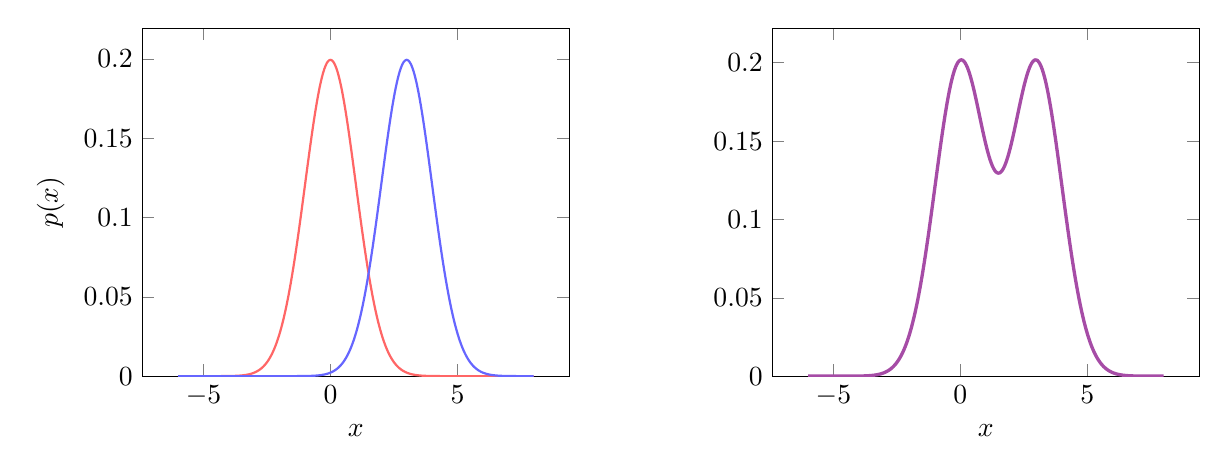
\begin{tikzpicture}

% ---------- Left plot: individual components ----------
\begin{axis}[
    at={(0,0)},
    anchor=south west,
    domain=-6:8,
    samples=300,
    width=7cm,
    height=6cm,
    xlabel={$x$},
    ylabel={$p(x)$},
    ymin=0,
    scaled y ticks=false,
    yticklabel style={
        /pgf/number format/fixed,
        /pgf/number format/precision=3
    }
]

% Soft red component
\addplot[
    thick,
    color=red!60
]
{0.5*(1/sqrt(2*pi)) * exp(-(x-0)^2/2)};

% Soft blue component
\addplot[
    thick,
    color=blue!60
]
{0.5*(1/sqrt(2*pi)) * exp(-(x-3)^2/2)};

\end{axis}

% ---------- Right plot: mixture ----------
\begin{axis}[
    at={(8cm,0)},
    anchor=south west,
    domain=-6:8,
    samples=300,
    width=7cm,
    height=6cm,
    xlabel={$x$},
    ymin=0,
    scaled y ticks=false,
    yticklabel style={
        /pgf/number format/fixed,
        /pgf/number format/precision=3
    }
]

% Soft purple mixture
\addplot[
    very thick,
    color=violet!70
]
{0.5*(1/sqrt(2*pi)) * exp(-(x-0)^2/2)
 +0.5*(1/sqrt(2*pi)) * exp(-(x-3)^2/2)};

\end{axis}

\end{tikzpicture}


This allows GMMs to model complex distributions that cannot be captured by a single normal distribution. Note that if we simply added two Gaussian densities together, the total area under the curve would be 2, so the result would no longer be a valid probability density. In a Gaussian mixture model, we instead take weighted proportions of each component, with weights that sum to 1. This ensures that the overall mixture still integrates to 1 and remains a proper probability distribution.

\bigskip

\subsection{Parameter Estimation via the EM Algorithm}

\medskip

The parameters of a Gaussian Mixture Model are typically estimated using the \emph{Expectation–Maximization} (EM) algorithm. Because the component labels are unobserved (we do not know which Gaussian generated each data point), direct maximization of the likelihood is not straightforward. The EM procedure addresses this difficulty by alternating between estimating cluster memberships and updating the model parameters.

\medskip

The algorithm proceeds as follows:

\begin{enumerate}[itemsep=0.8em]
    \item \textbf{Initialization.}
    Choose initial values for the parameters
    \[
    \{\mu_k, \Sigma_k, \pi_k\}_{k=1}^K.
    \]
    These may be selected randomly or obtained from a simpler
    clustering method such as $K$-means. Since the likelihood is not
    globally concave, initialization can influence the final solution.

    \item \textbf{Expectation Step (E-step).}
    Using the current parameter values, compute the probability that
    each observation belongs to each component. For each data point
    $x_i$, this produces a set of posterior probabilities that sum to 1.
    These values quantify soft cluster membership.

    \item \textbf{Maximization Step (M-step).}
    Update the parameters $\mu_k$, $\Sigma_k$, and $\pi_k$ so as to
    maximize the likelihood of the observed data, given the current
    membership probabilities. In effect, the parameters are re-estimated
    using weighted versions of the data.

    \item \textbf{Convergence.}
    Repeat the E-step and M-step until the parameter estimates stabilize
    or the increase in log-likelihood becomes negligible.
\end{enumerate}

Thus, EM alternates between estimating latent structure (cluster
membership probabilities) and optimizing the parameters conditional
on that structure. The procedure produces a sequence of parameter
estimates with non-decreasing likelihood, converging to a local maximum.

\bigskip

\subsection{Applications \& Limitations}

\medskip

GMM has applications in areas with complex data, such as speech recognition, finance, and image processing. The limitations of GMM include:

\begin{enumerate}[itemsep=0.5em]
    \item \textbf{Gaussian component assumption.} 
    GMM assumes the data are generated from a finite mixture of Gaussian components, 
    which implies ellipsoidal cluster shapes. If the true structure is strongly 
    non-Gaussian or heavy-tailed, the model may fit poorly or require many components.

    \item \textbf{Computational cost.} 
    The EM algorithm can be computationally expensive, especially in 
    high-dimensional settings where estimating full covariance matrices 
    scales poorly with dimension.

    \item \textbf{Sensitivity to initialization.} 
    The EM algorithm converges to a local maximum of the likelihood. 
    As a result, different initializations can lead to different solutions.

    \item \textbf{Choice of number of components.} 
    The number of mixture components $K$ is not determined automatically 
    and must be selected using model selection criteria such as BIC or AIC.
\end{enumerate}


\section{DBSCAN Advanced Cluster Analysis}

\medskip

Some key R commands are:
\begin{itemize}
    \item \texttt{db <- dbscan(data, eps = eps, minPts = minPts)}: the main function call. Here, \texttt{eps} (epsilon) is the fixed radius of the neighborhoods in which DBSCAN searches for dense regions, and \texttt{minPts} is the minimum number of points required within that radius (including the point itself) for a point to be considered a core point.

    \item \texttt{kNNdistplot(data, k = k)}: produces a $k$-nearest neighbor distance plot. For each point, the distance to its $k$th nearest neighbor is computed and plotted in sorted order. This is commonly used to help choose a reasonable value for \texttt{eps}. A sharp change or ``elbow'' in the plot often suggests a good cutoff for the neighborhood radius.

    \item \texttt{table(db\$cluster)}: tabulates the number of points assigned to each cluster. In the output, cluster labels are given as integers, and points labeled as \texttt{0} correspond to noise (points not assigned to any cluster).
\end{itemize}

\medskip


Density-Based Spatial Clustering of Applications with Noise (DBSCAN) is a clustering method based on the idea that clusters are regions of high point density separated by regions of low density. Unlike methods such as $k$-means, DBSCAN can explicitly classify observations as:

\begin{itemize}[label=--]
    \item Core: points whose $\epsilon$-neighborhood (including the point itself) contains at least \texttt{minPts} points.
    \item Boundary: points that are not core points but lie within the $\epsilon$-neighborhood of a core point.
    \item Noise: points that are neither core nor boundary, and therefore do not belong to any cluster.
\end{itemize}

DBSCAN does not assume any underlying probability distribution. Instead, it identifies clusters purely through geometric density, using $\epsilon$ as a distance threshold and \texttt{minPts} as a minimum local density requirement.


\bigskip

\subsection{How the Algorithm Works}

\medskip

\begin{enumerate}[itemsep=0.5em]
    \item A data point is selected and the number of points within $\epsilon$ of it is counted. If its $\epsilon$-neighborhood (including the point itself) contains at least \texttt{minPts} points, it is classified as a ``core'' point and used as a seed for a new cluster. Otherwise, it is temporarily labeled as noise.
    
    \item The cluster is expanded by adding all points within $\epsilon$ of the seed (these points are density-reachable from the seed).
    
    \item For each point added to the cluster, if it is also a core point, then all of its $\epsilon$-neighbors are added as well. This process continues until no new density-reachable points can be added.
    
    \item Once the cluster stops growing, a new unvisited point is selected and tested to determine whether it can start another cluster.
    
    \item After all points have been processed, any point not assigned to a cluster is labeled as noise.
\end{enumerate}

This allows DBSCAN to form clusters with complex shapes by chaining together regions of high density. Compared to $k$-means, DBSCAN does not penalize points that are far apart in the same cluster, as long as there is a sufficiently dense ``path'' of points connecting them.

\bigskip

\subsection{Advantages, Applications, \& Limitations}

\medskip

The key advantages of DBSCAN are the flexibility it provides in defining density requirements through \texttt{eps} and \texttt{minPts}, its ability to explicitly identify noise points, and its capacity to recover clusters with arbitrary, non-convex shapes. Unlike $k$-means, it does not require specifying the number of clusters in advance. DBSCAN has wide applications in geospatial analysis, image processing, anomaly detection, and customer segmentation.

Key limitations of DBSCAN are its sensitivity to the choice of parameters, particularly \texttt{eps}. Small changes in \texttt{eps} can substantially alter the clustering structure. In addition, DBSCAN uses a single global $\epsilon$ value, which makes it difficult to correctly identify clusters that have different densities or widths within the same dataset. In high-dimensional settings, distance measures become less informative due to the curse of dimensionality, which can make density-based neighborhood definitions unreliable. Finally, DBSCAN can struggle when clusters are very close together, as it may incorrectly merge them if their high-density regions connect.

\bigskip

\subsection{Choosing Parameter Values}

\medskip

Since the choice for the parameters significantly affects the output, we should consider some rules of thumb:
\begin{itemize}[label=--, itemsep=0.7em]
    \item \texttt{minPts} = $p + 1$, where $p$ is the number of features. 
    \begin{itemize}[label=$\circ$, itemsep=0.3em]
        \item This is a theoretical lower bound: in $p$-dimensional space, at least $p+1$ points are required to form a full-dimensional simplex (the smallest set of points that spans the entire $p$-dimensional space rather than lying in a lower-dimensional subspace). 
        \item With fewer than $p+1$ points, observations can lie on a lower-dimensional manifold and spuriously appear dense, so DBSCAN may identify unstable or degenerate clusters. Thus $p+1$ is the smallest value that meaningfully defines local density in $p$-space, but it is rarely sufficient in practice.
    \end{itemize}
    
    \item \texttt{minPts} = $2p$
    \begin{itemize}[label=$\circ$, itemsep=0.3em]
        \item This is a common heuristic that increases the minimum neighborhood size to make density estimates more stable and less sensitive to noise. However, it is not theoretically justified: the appropriate value depends on the intrinsic dimensionality, the noise level, and the actual spatial distribution of the data.
        \item In higher dimensions or noisy datasets, substantially larger values may be required.
    \end{itemize}
    \item Experiment with a range of $\epsilon$ and \texttt{minPts} (grid search)
    \item Use relevant domain knowledge for the subject
    \item Use a \textit{k-distance graph}.
\end{itemize}

\medskip

\subsubsection{k-distance Graphs}

\medskip

This is used to \textit{refine} $\epsilon$ once we already have a tentative value for \texttt{minPts}. The idea is as follows:

\begin{enumerate}
    \item For each data point, compute the distance to its $k$th nearest neighbor, where $k$ is the chosen value for \texttt{minPts}. We record only this $k$th distance, since it represents the smallest radius needed for the point to have at least \texttt{minPts} neighbors. Distances to closer points are not needed for this diagnostic.

    \item Collect all of these $k$-nearest neighbor distances and sort them from smallest to largest.
    
    \item Plot the ordered distances against their index (from $1$ to $n$). The resulting curve will be non-decreasing (monotonically increasing).
\end{enumerate}

\medskip

To choose $\epsilon$, look for a noticeable ``elbow'' in the curve. The distance value at this elbow is often a good choice for $\epsilon$. Intuitively, the elbow marks the transition between points in dense regions (small $k$-distances) and points in sparser regions or noise (rapidly increasing $k$-distances).


\section{Outliers}

\medskip

An outlier is a case/observation that is not typical of the rest of the data. There are several different ways that we could ways we could define what an outlier is for a given dataset. For example, we could define it as any point $> 2 \sigma$ away from the mean. With this definition, there isn't anything necessarily ``wrong" with an outlier. In fact, if the data were normally distributed we would expect ~ 4\% of the data to be outliers. The following table compares some different ways to define an outlier for a given dataset.

\begin{table}[H]
\centering
\renewcommand{\arraystretch}{1.5}
\rowcolors{2}{gray!10}{white}
\begin{tabularx}{0.95\textwidth}{
l
>{\hsize=1.1\hsize}X
>{\hsize=0.9\hsize}X
}
\toprule
\textit{Meaning} 
& \textit{Definition / Key Idea} 
& \textit{Features (Advantage / Disadvantage)} \\
\midrule
Absolute standard 
& A value that exceeds a fixed cutoff (e.g., 2 or more standard deviations from the mean). 
The expected number of such values increases with sample size. 
& + Simple and easy to apply \newline
-- Ignores sample size effects and distributional context \\

Relative standard 
& A value that exceeds what would reasonably be expected given the size of the dataset. 
Outlier status depends on sample size and probabilistic expectations. 
& + Adjusts for sample size and randomness \newline
-- Requires distributional assumptions \\

Objective standard 
& A value known not to belong for an external, substantive reason 
(e.g., drawn from a different population). 
& + Grounded in subject-matter knowledge \newline
-- May rely on unverifiable or subjective judgment \\

Effect 
& A value whose inclusion or exclusion substantially changes the analysis 
(e.g., regression slope, parameter estimates, or conclusions). 
& + Directly tied to inferential impact \newline
-- Identified only after model fitting, can be circular \\
\bottomrule
\end{tabularx}
\caption*{Four Meanings of an Outlier}
\end{table}

When defining outliers based on their effect on a regression, what we are really identifying are \textit{influential observations}. We check whether removing a point meaningfully changes the fitted model, including the slope coefficients, the intercept, or fit statistics such as $R^2$. A noticeable change in any of these suggests influence.

Influence itself is not inherently bad. In fact, influential observations often carry much of the information that determines the fitted relationship. Points that have no influence simply do not affect the model. The real concern is whether the influential observations are “good” data, meaning correctly measured and representative of the population of interest.

In regression, an observation may be unusual in the predictor space (an outlier in $X$), unusual in the response (an outlier in $Y$), both, or neither. Not all such points are influential. Some extreme observations have little effect on the fitted line, while others, particularly high-leverage points, can substantially shift the estimates. For this reason, observations cannot be treated uniformly under this definition. Unlike the other approaches, this perspective classifies points based on their impact on the analysis rather than their magnitude or origin.

\bigskip

\subsection{Dealing with Outliers}

\medskip

For highly (inappropriately) influential outliers, we may choose the drastic option of dropping (removing) the data point entirely. This approach needs strong justification because it assumes that your model choice is correct and that the data is wrong. In many data sets, the reality may be that the model is insufficiently capturing the information in the data. 

Another approach is to keep them, but to turn them into binary variables (if we are doing a regression). This treats the influential point as a special case rather than allowing it to distort the overall relationship.

\bigskip

\subsection{Isolation Forest}

\medskip

Some key R commands are:
\begin{itemize}
    \item \texttt{library(isotree)}: Loads the \texttt{isotree} package, which implements IF and EIF.

    \item \texttt{isolation.forest()}: Fits an Isolation Forest (or Extended IF) model to the data.

    With key parameters:
    \begin{itemize}[label=$\circ$, itemsep=0.3em]
        \item \texttt{ntrees}: Number of trees in the forest (default 100).
        \item \texttt{sample\_size}: Number of observations used to train each tree (default is ``auto'', typically $\min(256, n)$).
        \item \texttt{ndim}: Number of features used per split; \texttt{ndim = 1} gives standard IF, \texttt{ndim > 1} gives EIF.
        \item \texttt{max\_depth}: Maximum tree depth (default ``auto'', allowing full isolation).
        \item \texttt{nthreads}: Number of CPU threads for parallel computation (default 1).
        \item \texttt{missing\_action}: How to handle missing values (e.g., ``fail'', ``impute'', or ``divide'').
    \end{itemize}
\end{itemize}

\medskip


The way Isolation Forest (IF) works is that, similar in structure to a decision tree, it repeatedly makes \textit{random axis-aligned hyperplane partitions} of the data. “Axis-aligned” means that each split involves only one feature at a time, so in two dimensions these would look like vertical or horizontal cuts, and in higher dimensions they are coordinate-wise hyperplane splits of the form $x_j=c$. Importantly, unlike standard decision trees, these splits are not chosen greedily to optimize a criterion, both the feature and the split point are selected at random.

This recursive partitioning continues until a data point is isolated in its own node, or until a maximum tree depth is reached. For each observation, we record the number of splits required to isolate it, known as its \textit{path length}, and average this quantity across many random trees. Observations that require substantially fewer splits to isolate, meaning they have shorter average path lengths, are labeled as outliers.

The underlying idea is that anomalies should be both rare and different from the bulk of the data. Because they are isolated in sparse regions of the feature space, random partitions tend to separate them more quickly than typical observations.

\bigskip

\subsubsection{IF Algorithm}

\medskip

An Isolation Forest consists of many independently constructed isolation trees. 
Each tree is grown on a random subsample of the data, which increases variability across trees and stabilizes the final anomaly score through averaging.

Within a single tree, the recursive splitting process continues across all branches until observations are isolated in terminal nodes (or a predefined maximum depth is reached). 
The result is a random partitioning of the feature space into progressively smaller regions. 
Because splits are random rather than optimized, the structure of any single tree is not meaningful on its own, only the aggregated behavior across many trees is informative.

For each observation, we compute its \textit{path length}, defined as the number of splits required to travel from the root node (the full dataset) to the terminal leaf containing that observation. This path length is averaged over the ensemble. Short average path lengths indicate that the observation consistently falls into small, sparse regions of the feature space, whereas longer paths indicate that the point lies in denser regions and is harder to isolate.

Thus, the anomaly score is fundamentally a measure of how quickly random recursive partitioning separates a point from the rest of the data.


\medskip

\textbf{Anomaly Score}

Formally, the anomaly score $s(x,n)$ for a point $x$ in a dataset of size $n$ is defined as
\[
s(x,n) = 2^{-\frac{E(h(x))}{c(n)}},
\]
where:

\begin{itemize}
    \item $h(x)$ is the path length of $x$ in a single isolation tree, that is, the number of splits required to isolate $x$.
    \item $E(h(x))$ is the average path length of $x$ across all trees in the ensemble.
    \item $c(n)$ is a normalizing constant representing the average path length of an unsuccessful search in a random binary search tree of size $n$. 
    That is, it approximates the expected depth of a point under purely random binary partitioning, providing a baseline for how many splits it should take to isolate a typical observation.

\end{itemize}

The quantity $c(n)$ can be approximated by
\[
c(n) = 2H(n-1) - \frac{2(n-1)}{n},
\]
where $H(i)$ is the $i$th harmonic number,
\[
H(i) = \sum_{k=1}^{i} \frac{1}{k}.
\]

The harmonic number appears because the expected depth of a node in a randomly constructed binary search tree grows proportionally to $H(n)$. 
Since $H(n) \approx \log(n)$ for large $n$, this reflects the fact that under random splitting, the expected number of partitions needed to isolate a typical point grows roughly logarithmically with the dataset size. 
Thus, $c(n)$ provides a baseline for how long paths are expected to be purely due to sample size and random partitioning.

The ratio $\frac{E(h(x))}{c(n)}$ therefore measures how the observed path length of $x$ compares to what we would expect for a typical point in a dataset of size $n$. 
Values smaller than 1 indicate that $x$ is isolated more quickly than expected, while values near or above 1 indicate typical or longer-than-expected isolation.

The exponential form $2^{-\frac{E(h(x))}{c(n)}}$ rescales this quantity to lie between 0 and 1 in a smooth and monotonic way. 
Because isolation trees are binary, path lengths naturally scale in powers of 2, so the base 2 transformation is consistent with the tree structure. 
Shorter path lengths produce scores close to 1, while longer path lengths push the score toward 0.

Intuitively, the anomaly score answers the question: 
\emph{How quickly does random recursive partitioning separate this point from the rest of the data, relative to what we would expect under random structure?} 
Points that are isolated unusually quickly are considered anomalous because they lie in sparse or distinct regions of the feature space.

\bigskip

\subsubsection{Extended Isolation Forest}

\medskip

Extended Isolation Forest (EIF) is a modification of the original Isolation Forest. Instead of only making splits perpendicular to the axes, EIF uses more general hyperplanes to partition the data.

It achieves this by selecting a random subset of features and generating a random linear combination to define a splitting hyperplane. This allows partitions that are not constrained to be parallel to coordinate axes. The rest of the procedure is the same: trees are built via recursive random partitioning, and anomaly scores are computed using average path length. 

The advantage of EIF is that the more flexible hyperplanes can better adapt to the geometry of the data, which often leads to more effective isolation of anomalies in high-dimensional settings.

\medskip

\begin{table}[H]
\centering
\renewcommand{\arraystretch}{1.5}
\rowcolors{2}{gray!10}{white}
\begin{tabularx}{0.95\textwidth}{
>{\raggedright\arraybackslash}p{0.18\textwidth}
X
X
}
\toprule
\textit{Method} 
& \textit{Partitioning Strategy} 
& \textit{Features} \\
\midrule
Isolation Forest (IF) 
& Uses random axis-aligned hyperplane splits (perpendicular to a single feature axis at each partition). 
& + Simpler and computationally efficient \newline
-- Can be limited when structure is not aligned with coordinate axes \\

Extended Isolation Forest (EIF) 
& Uses randomly oriented hyperplanes, allowing splits at arbitrary angles in the feature space. 
& + More flexible partitioning \newline
+ More effective anomaly detection in high-dimensional data \newline
-- Increased computational complexity \newline
-- Greater parameter sensitivity (e.g., number of features used per split) \\
\bottomrule
\end{tabularx}
\caption*{Comparison of Isolation Forest and Extended Isolation Forest}
\end{table}


\section{Clustering in High Dimensions}

\medskip

High-dimensional data introduce both computational and geometric difficulties. 
Computationally, resource requirements can grow exponentially in the number of features $p$ (e.g., checking all subsets in regression requires $2^p$ models). Geometrically, the problem becomes qualitatively different: distances between points lose contrast. Since clustering methods such as K-means rely directly on distances, this phenomenon undermines their effectiveness.

\medskip

\textbf{Distance concentration.}

Let $x_i, x_j \in \mathbb{R}^p$ have independent standard normal coordinates. The squared Euclidean distance is
\[
\|x_i - x_j\|^2 = \sum_{k=1}^p (x_{ik} - x_{jk})^2.
\]
Each coordinate difference has variance $2$, so
\[
\mathbb{E}\big[\|x_i - x_j\|^2\big] = 2p.
\]
Moreover,
\[
\frac{\text{stdev}\big(\|x_i - x_j\|^2\big)}{\mathbb{E}\big(\|x_i - x_j\|^2\big)} 
= \frac{\sqrt{2p}}{2p}
= \frac{1}{\sqrt{p}}
\to 0 \quad \text{as } p \to \infty.
\]
The ratio above is the \emph{coefficient of variation}, which measures relative dispersion. 
As $p$ increases, the relative spread of distances shrinks. Distances grow in magnitude, but their \emph{relative variability} vanishes. In high dimensions, most pairwise distances are nearly the same. This “flattening” of geometry makes distance-based clustering fragile.

\medskip

\textbf{PCA before clustering.}

A standard remedy is to reduce dimension using Principal Components Analysis (PCA) and then cluster in the reduced subspace. If $X$ is a centered $n \times p$ data matrix, PCA computes
\[
S = \frac{1}{n-1} X^\top X, \qquad
S = V \Lambda V^\top, \qquad
Z = XV.
\]
The first $K$ principal components,
\[
Z_{1:K} = X V_{1:K},
\]
span directions of maximal variance. By projecting onto these directions, we often remove noise and collinearity while preserving dominant structure. Clustering is then performed on $Z_{1:K}$ rather than on the original $p$-dimensional space. Note that PCA maximizes variance, not class separation. High explained variance does not guarantee well-separated clusters.

\medskip

\textbf{Evaluating clustering performance.}

When true labels are available (e.g., case studies), we can use external validation metrics.

\emph{Adjusted Rand Index (ARI).}

ARI compares a clustering to known labels. It equals 1 for perfect agreement and has expected value 0 under random partitions. Moderate ARI values (e.g., 0.2–0.5) can still indicate meaningful structure in unsupervised settings.

A low ARI does not necessarily imply useless clusters. For example, in IoT flow data, labels may represent very specific attack categories, while K-means discovers broader traffic regimes (e.g., bursty vs steady behavior). The geometric structure found by clustering may not align with the semantic labeling scheme.

\emph{Jaccard index.}
When no ground-truth labels exist, we may compare two clusterings using pairwise co-membership overlap:
\[
J(A,B) = \frac{|A \cap B|}{|A \cup B|}.
\]

Intuitively, Jaccard answers the question: \emph{of all the pairs of observations that at least one clustering puts together, what fraction do both clusterings agree on?}

Think in terms of pairs of data points. For any two observations, there are two possibilities in a given clustering: either they are placed in the same cluster (co-membership) or they are not. For two clusterings $A$ and $B$:

\begin{itemize}[label=$\circ$, itemsep=0.3em]
    \item $|A \cap B|$ counts the number of pairs that \emph{both} clusterings place in the same cluster.
    \item $|A \cup B|$ counts the number of pairs that \emph{at least one} clustering places in the same cluster.
\end{itemize}

Thus, the Jaccard index measures the proportion of shared grouping decisions among all grouping decisions made by either clustering. 

A value close to 1 means the two clusterings group essentially the same pairs together. A value near 0 means that when one clustering groups two observations together, the other typically does not.

Because it only compares clusterings to each other, Jaccard is useful for assessing \emph{stability}: for example, re-running K-means with different random starts or on bootstrap samples and checking whether the resulting partitions are consistent.

\medskip

\textbf{Feature selection and sparsity.}

If we prefer not to project onto principal components, we may instead reduce dimensionality by selecting or weighting features.

\emph{Filter methods.}
Rank variables by variance, mutual information, or univariate tests, and retain the top $m$. These methods are computationally simple and interpretable but ignore feature interactions.

\emph{Embedded sparsity (e.g., sparse K-means).}
Some methods learn feature weights directly during clustering:
\[
\max_{\{C_k\}, w} \sum_{j=1}^p w_j \, \text{BCSS}_j 
\quad \text{s.t.} \quad 
\sum_{j=1}^p |w_j| \le \tau, 
\quad w_j \ge 0.
\]
Here $\text{BCSS}_j$ is the between-cluster sum of squares for feature $j$, and $w_j$ are nonnegative weights constrained by a budget $\tau$. The constraint induces sparsity, concentrating weight on a subset of discriminative variables and down-weighting noisy dimensions.

\medskip

\textbf{Common misconceptions of high-dimensional clustering are:}
\begin{itemize}[label=$\circ$, itemsep=0.4em]
    \item More features help $\longrightarrow$ Not necessarily true. Adding weak or noisy variables increases distance concentration and can blur cluster structure in distance-based methods.
    \item High explained variance guarantees good clusters $\longrightarrow$ PCA maximizes variance, not class separation. A small set of PCs can explain most variance yet still fail to separate groups.
    \item K-means failed so there are no clusters $\longrightarrow$ K-means searches for roughly spherical clusters under Euclidean distance. Non-spherical or density-based structure may require alternative methods (e.g., DBSCAN or hierarchical clustering).
    \item Only ARIs near 1 are useful $\longrightarrow$ In real unsupervised problems, moderate ARI values (e.g., 0.2--0.5) can still reflect meaningful and managerially useful segmentation.
\end{itemize}


\section{Association Rules}

\medskip

Association rules (AR) describe patterns in which certain items tend to occur together in transactional data. Association rule learning discovers such co-occurrence patterns and evaluates their strength.

Consider the rule
\[
\{bread, butter\} \implies \{milk\}.
\]
This means that transactions containing bread and butter are often associated with milk. An \emph{itemset} is simply a collection of items that appear together in a transaction.

Association rule learning proceeds in two main steps:
\begin{itemize}
    \item Frequent itemset generation (identify itemsets that occur often enough in the data)
    \item Rule generation (form rules from frequent itemsets and evaluate them using measures of strength)
\end{itemize}

\medskip

We briefly recall some set operations. For two sets $A$ and $B$:
\begin{itemize}
    \item The union is $A \cup B$
    \item The intersection is $A \cap B$
\end{itemize}

If we know the counts of $A$, $B$, and $A \cap B$, then the count of the union is
\[
|A \cup B| = |A| + |B| - |A \cap B|.
\]
This subtracts the double-counted intersection.

\medskip

The \emph{support} of an itemset $X$ is the proportion of transactions in which $X$ appears:
\[
\text{Support}(X) = \frac{\#\text{ transactions containing } X}{\#\text{ total transactions}}.
\]
Support can be interpreted as the unconditional probability $P(X)$.

\medskip

The \emph{confidence} of a rule $X \implies Y$ measures how often $Y$ appears in transactions that already contain $X$:
\[
\text{Confidence}(X \implies Y)
=
\frac{\#(X \cap Y)}{\#(X)}
=
P(Y \mid X).
\]
Confidence is a conditional probability. It is not symmetric: in general,
\[
P(Y \mid X) \neq P(X \mid Y).
\]

\medskip

The \emph{lift} of a rule compares the observed co-occurrence of $X$ and $Y$ to what would be expected if they were independent:
\[
\text{Lift}(X \implies Y)
=
\frac{\text{Confidence}(X \implies Y)}{\text{Support}(Y)}
=
\frac{P(Y \mid X)}{P(Y)}.
\]

Lift measures departure from independence:
\begin{itemize}
    \item Lift $= 1$ $\longrightarrow$ $X$ and $Y$ are independent
    \item Lift $> 1$ $\longrightarrow$ positive association
    \item Lift $< 1$ $\longrightarrow$ negative association
\end{itemize}

Lift is always nonnegative. It measures relative increase in probability, not odds.

\bigskip

\subsection{apriori()}

\medskip

The \texttt{apriori()} algorithm is a classical method for association rule learning. Its goal is to efficiently identify \emph{frequent itemsets} and then generate strong rules from them. The key idea is the \textit{Apriori property}:
\[
\text{If an itemset is frequent, then all of its subsets must also be frequent.}
\]
Equivalently, if a subset of an itemset is infrequent, then the larger itemset cannot possibly be frequent. This allows the algorithm to aggressively prune the search space.

\medskip

The algorithm proceeds iteratively:
\begin{itemize}
    \item Start by finding all frequent 1-itemsets (items whose support exceeds the minimum threshold).
    \item Use these to generate candidate 2-itemsets.
    \item Prune any candidate whose subsets are not frequent.
    \item Repeat for 3-itemsets, 4-itemsets, and so on, until no further frequent itemsets are found.
\end{itemize}

This is a breadth-first search over itemset size. At each stage, only candidates that satisfy the Apriori property are retained, dramatically reducing computation.

\medskip

The data must be in transactional form. Each row represents a transaction (e.g., a basket), and each transaction is a set of items. In R, this is typically stored as a \texttt{transactions} object from the \texttt{arules} package.

\medskip

\textbf{Key parameters in \texttt{apriori()}:}
\begin{itemize}[label=$\circ$, itemsep=0.4em]
    \item Support $\longrightarrow$ Minimum support threshold for an itemset to be considered frequent.
    \item Confidence $\longrightarrow$ Minimum confidence threshold for a rule to be retained.
    \item Lift $\longrightarrow$ Used to assess strength beyond random co-occurrence.
\end{itemize}

Support controls how common a pattern must be. Confidence controls how reliable the implication $X \implies Y$ must be. Lift evaluates whether the rule represents genuine association rather than chance.

\medskip

\textbf{Output and visualization.}

The output consists of a set of association rules satisfying the specified thresholds. These can be visualized using the \texttt{arulesViz} package. Common visualizations include:
\begin{itemize}[label=$\circ$, itemsep=0.4em]
    \item Scatter plots $\longrightarrow$ Displaying support, confidence, and lift of rules.
    \item Matrix plots $\longrightarrow$ Showing support relationships among itemsets.
    \item Graph-based plots $\longrightarrow$ Representing rules as a network of items.
\end{itemize}

The central trade-off is computational: lower support thresholds increase rule discovery but dramatically expand the candidate search space.

\bigskip

\subsection{Advantages \& Disadvantages}

\medskip

The advantages of ARL are that it is easy to both understand and implement, the generated rules are easy to interpret, and that some algorithms (a priori) are efficient and can therefore be scaled for large datasets. 

The disadvantages are that generating datasets of frequent items can be expensive, some generated rules can be redundant or uninteresting, and that the method is highly sensitive to the parameter choice (cut-offs for support and confidence thresholds).



\newpage
\section{Worked Examples}

\bigskip

\subsection{PCA with Two Variables}
\label{worked-pca-two-variables}

This example illustrates the transition from original variables to principal components using a bivariate dataset.

\medskip

\begin{enumerate}
    \setlength{\itemsep}{1em}
    
    \item \textit{Original Data}: Suppose we have the following observations for variables $X_1$ and $X_2$:

    \[
    \mathbf{X} =
    \begin{bmatrix}
    2 & 3 \\
    4 & 5 \\
    5 & 7 \\
    3 & 4
    \end{bmatrix}
    \]

    \item \textit{Standardizing the Data}: Standardize each variable to have mean 0 and standard deviation 1:

    \[
    Z_1 = \frac{X_1 - \bar{X}_1}{s_{X_1}}, \quad
    Z_2 = \frac{X_2 - \bar{X}_2}{s_{X_2}}
    \]

    Compute means and standard deviations:

    \[
    \bar{X}_1 = \frac{2+4+5+3}{4} = 3.5, \quad
    \bar{X}_2 = \frac{3+5+7+4}{4} = 4.75
    \]
    
    \[
    s_{X_1} = \sqrt{\frac{(2-3.5)^2 + (4-3.5)^2 + (5-3.5)^2 + (3-3.5)^2}{4-1}} \approx 1.29
    \]
    
    \[
    s_{X_2} = \sqrt{\frac{(3-4.75)^2 + (5-4.75)^2 + (7-4.75)^2 + (4-4.75)^2}{3}} \approx 1.71
    \]

    Standardized matrix:

    \[
    \mathbf{Z} =
    \begin{bmatrix}
    -1.16 & -1.03 \\
     0.39 & 0.15 \\
     1.16 & 1.31 \\
    -0.39 & -0.22
    \end{bmatrix}
    \]

    Total variance of standardized variables: $1+1=2$.

    \item \textit{Correlation Matrix}: Compute the correlation (equivalent to covariance for standardized data):
    
    The correlation between $Z_1$ and $Z_2$ is
    
    \[
    r_{12} = \frac{1}{n-1} \sum_{i=1}^{n} Z_{1i} Z_{2i}
    \]
    
    Step by step multiplication:
    
    \[
    Z_1 Z_2 =
    \begin{bmatrix}
    (-1.16)(-1.03) = 1.1948 \\
    (0.39)(0.15) = 0.0585 \\
    (1.16)(1.31) = 1.5196 \\
    (-0.39)(-0.43) = 0.1677
    \end{bmatrix}
    \]
    
    Sum:
    
    \[
    1.1948 + 0.0585 + 1.5196 + 0.1677 \approx 2.9406
    \]
    
    Divide by $n-1 = 3$:
    
    \[
    r_{12} = \frac{2.9406}{3} \approx 0.9802
    \]
    
    Correlations of variables with themselves are 1, so the correlation matrix is
    
    \[
    \mathbf{R} =
    \begin{bmatrix}
    1 & 0.980 \\
    0.980 & 1
    \end{bmatrix}
    \]
    
    \item \textit{Eigenvalues and Eigenvectors}:
    
    Solve the characteristic equation
    
    \[
    \det(\mathbf{R} - \lambda \mathbf{I}) = 0
    \]
    
    Step by step:
    
    \[
    \begin{vmatrix}
    1-\lambda & 0.980 \\
    0.980 & 1-\lambda
    \end{vmatrix} = (1-\lambda)(1-\lambda) - (0.980)^2 = 0
    \]
    
    \[
    (1-\lambda)^2 - 0.9604 = 0
    \]
    
    \[
    (1-\lambda)^2 = 0.9604 \implies 1-\lambda = \pm 0.980
    \]
    
    \[
    \lambda_1 = 1 + 0.980 = 1.980, \quad \lambda_2 = 1 - 0.980 = 0.020
    \]
    
    Eigenvectors:
    
    For $\lambda_1 = 1.980$:
    
    \[
    (\mathbf{R} - \lambda_1 \mathbf{I})\mathbf{v}_1 =
    \begin{bmatrix}
    1-1.980 & 0.980 \\
    0.980 & 1-1.980
    \end{bmatrix} 
    \begin{bmatrix} v_{11} \\ v_{12} \end{bmatrix} =
    \begin{bmatrix}
    -0.980 & 0.980 \\
    0.980 & -0.980
    \end{bmatrix}
    \begin{bmatrix} v_{11} \\ v_{12} \end{bmatrix} = 0
    \]
    
    Solving $-0.980 v_{11} + 0.980 v_{12} = 0 \implies v_{11} = v_{12}$. Normalize:
    
    \[
    \mathbf{v}_1 = \frac{1}{\sqrt{2}}
    \begin{bmatrix} 1 \\ 1 \end{bmatrix} =
    \begin{bmatrix} 0.707 \\ 0.707 \end{bmatrix}
    \]
    
    For $\lambda_2 = 0.020$:
    
    \[
    v_{21} = -v_{22} \implies
    \mathbf{v}_2 = \frac{1}{\sqrt{2}}
    \begin{bmatrix} 1 \\ -1 \end{bmatrix} =
    \begin{bmatrix} 0.707 \\ -0.707 \end{bmatrix}
    \]


    Eigenvectors (normalized):

    \[
    \mathbf{v}_1 = 
    \begin{bmatrix}
    0.707 \\
    0.707
    \end{bmatrix}, \quad
    \mathbf{v}_2 =
    \begin{bmatrix}
    0.707 \\
    -0.707
    \end{bmatrix}
    \]

    \item \textit{Forming Principal Components}: Each component is a linear combination of standardized variables:

    \[
    \xi_1 = 0.707 Z_1 + 0.707 Z_2, \quad
    \xi_2 = 0.707 Z_1 - 0.707 Z_2
    \]

    The first component explains $\frac{1.981}{2} \approx 99\%$ of the total variance.

    \item \textit{Verifying Orthonormality}:

    \[
    0.707^2 + 0.707^2 \approx 0.5 + 0.5 = 1
    \]

    \item \textit{Calculating Component Scores} (coordinates of the original data in the new PC space):

    \[
    \mathbf{\Xi} = \mathbf{Z} \mathbf{V} =
    \begin{bmatrix}
    -1.46 & -0.09 \\
     0.38 & -0.04 \\
     1.82 & 0.07 \\
    -0.74 & 0.05
    \end{bmatrix}
    \]

    Here, the first column is $\xi_1$, the second is $\xi_2$.

    \item \textit{Reconstructing Original Variables}:

    Using the first component only:

    \[
    Z_1 \approx 0.707 \xi_1, \quad Z_2 \approx 0.707 \xi_1
    \]

    Including both components:

    \[
    \mathbf{Z} = \xi_1 \mathbf{v}_1^\top + \xi_2 \mathbf{v}_2^\top
    \]

\end{enumerate}



\newpage


\subsection{MDS Example}
\label{worked-mds}

\medskip

Consider four objects with distance matrix
\[
\mathbf{\Delta}
=
\begin{pmatrix}
0 & 3 & 4 & 5 \\
3 & 0 & 5 & 6 \\
4 & 5 & 0 & 7 \\
5 & 6 & 7 & 0
\end{pmatrix}.
\]

\medskip
\noindent
\textbf{Step 1: Square the distances}

\medskip

Squaring each entry gives
\[
\mathbf{\Delta}^{(2)}
=
\begin{pmatrix}
0 & 9 & 16 & 25 \\
9 & 0 & 25 & 36 \\
16 & 25 & 0 & 49 \\
25 & 36 & 49 & 0
\end{pmatrix}.
\]

\medskip
\noindent
\textbf{Step 2: Construct the centering matrix}

\medskip

Since $n = 4$,
\[
\mathbf{J}
=
\mathbf{I}_4 - \frac{1}{4}\mathbf{1}\mathbf{1}^T.
\]

Because $\frac{1}{4}\mathbf{1}\mathbf{1}^T$ is a matrix of all $1/4$'s, we obtain
{
\renewcommand{\arraystretch}{1.5}
\[
\mathbf{J}
=
\begin{pmatrix}
\frac{3}{4} & -\frac{1}{4} & -\frac{1}{4} & -\frac{1}{4} \\
-\frac{1}{4} & \frac{3}{4} & -\frac{1}{4} & -\frac{1}{4} \\
-\frac{1}{4} & -\frac{1}{4} & \frac{3}{4} & -\frac{1}{4} \\
-\frac{1}{4} & -\frac{1}{4} & -\frac{1}{4} & \frac{3}{4}
\end{pmatrix}.
\]}

\medskip
\noindent
\textbf{Step 3: Compute row means, column means, and the grand mean}

\medskip

Row means of $\mathbf{\Delta}^{(2)}$:

\[
\bar{a}_{1\cdot} = \frac{0+9+16+25}{4} = 12.5
\]
\[
\bar{a}_{2\cdot} = \frac{9+0+25+36}{4} = 17.5
\]
\[
\bar{a}_{3\cdot} = \frac{16+25+0+49}{4} = 22.5
\]
\[
\bar{a}_{4\cdot} = \frac{25+36+49+0}{4} = 27.5
\]

Because the matrix is symmetric, the column means are the same.

The grand mean is
\[
\bar{a}_{\cdot\cdot}
=
\frac{1}{16}
\sum_{i,j} a_{ij}
=
\frac{80}{4}
=
20.
\]

\medskip
\noindent
\textbf{Step 4: Apply double centering and rescaling}

\medskip

Recall that
\[
b_{ij}
=
-\frac{1}{2}
\left(
a_{ij}
-
\bar{a}_{i\cdot}
-
\bar{a}_{\cdot j}
+
\bar{a}_{\cdot\cdot}
\right).
\]

We compute a few entries explicitly.

\medskip

Entry $(1,1)$:
\[
b_{11}
=
-\frac{1}{2}
\left(
0 - 12.5 - 12.5 + 20
\right)
=
-\frac{1}{2}(-5)
=
2.5.
\]

\medskip

Entry $(1,2)$:
\[
b_{12}
=
-\frac{1}{2}
\left(
9 - 12.5 - 17.5 + 20
\right)
=
-\frac{1}{2}(-1)
=
0.5.
\]

\medskip

Entry $(1,4)$:
\[
b_{14}
=
-\frac{1}{2}
\left(
25 - 12.5 - 27.5 + 20
\right)
=
-\frac{1}{2}(5)
=
-2.5.
\]

Carrying this out for all entries yields
\[
\mathbf{B}
=
\begin{pmatrix}
2.5 & 0.5 & -0.5 & -2.5 \\
0.5 & 7.5 & -2.5 & -5.5 \\
-0.5 & -2.5 & 12.5 & -9.5 \\
-2.5 & -5.5 & -9.5 & 17.5
\end{pmatrix}.
\]

\medskip
\noindent
\textbf{Step 5: Full eigen-decomposition of $\mathbf{B}$}

\medskip

The eigenvalues of $\mathbf{B}$ are approximately
\[
\lambda_1 = 25.4573, \quad
\lambda_2 = 11.6406, \quad
\lambda_3 = 2.9021, \quad
\lambda_4 \approx 0.
\]

Thus the diagonal matrix of eigenvalues is

\[
\mathbf{\Lambda}
=
\begin{pmatrix}
25.4573 & 0 & 0 & 0 \\
0 & 11.6406 & 0 & 0 \\
0 & 0 & 2.9021 & 0 \\
0 & 0 & 0 & 0
\end{pmatrix}.
\]

A corresponding orthonormal eigenvector matrix is

\[
\mathbf{V}
=
\begin{pmatrix}
-0.0621 & 0.1435 & -0.9445 & 0.2887 \\
-0.2334 & 0.8202 & 0.3365 & -0.4082 \\
-0.5738 & -0.5204 & 0.0031 & -0.5774 \\
0.7833 & -0.1869 & 0.0008 & -0.5774
\end{pmatrix}.
\]

\medskip
\noindent
\textbf{Step 6: Constructing the 2D configuration}

\medskip

We retain the first two eigenvalues and eigenvectors:

\[
\mathbf{\Lambda}_2
=
\begin{pmatrix}
25.4573 & 0 \\
0 & 11.6406
\end{pmatrix},
\qquad
\mathbf{V}_2
=
\begin{pmatrix}
-0.0621 & 0.1435 \\
-0.2334 & 0.8202 \\
-0.5738 & -0.5204 \\
0.7833 & -0.1869
\end{pmatrix}.
\]

Taking square roots of the eigenvalues,

\[
\mathbf{\Lambda}_2^{1/2}
=
\begin{pmatrix}
\sqrt{25.4573} & 0 \\
0 & \sqrt{11.6406}
\end{pmatrix}
=
\begin{pmatrix}
5.0455 & 0 \\
0 & 3.4118
\end{pmatrix}.
\]

The coordinate matrix is

\[
\mathbf{X}
=
\mathbf{V}_2 \mathbf{\Lambda}_2^{1/2}.
\]

Carrying out the multiplication yields

\[
\mathbf{X}
=
\begin{pmatrix}
-0.402 & 0.490 \\
-0.870 & 2.490 \\
-2.808 & -2.108 \\
4.081 & -0.872
\end{pmatrix}.
\]

\medskip
\noindent
\textbf{Recomputing Euclidean distances}

\medskip

We now verify that these coordinates reproduce the original distances.

\medskip

Distance between objects 1 and 2:
\[
\sqrt{
(-0.402 + 0.870)^2
+
(0.490 - 2.490)^2
}
=
\sqrt{
(0.468)^2 + (-2.000)^2
}
=
\sqrt{0.219 + 4}
=
\sqrt{4.219}
\approx 2.054.
\]

\medskip

Distance between objects 1 and 3:
\[
\sqrt{
(-0.402 + 2.808)^2
+
(0.490 + 2.108)^2
}
=
\sqrt{
(2.406)^2 + (2.598)^2
}
=
\sqrt{5.791 + 6.752}
=
\sqrt{12.543}
\approx 3.543.
\]
This does not exactly match the original distance of 4.
The discrepancy is not merely rounding error. It arises because we
retained only the first two eigenvalues when constructing the
configuration.

Recall that $\mathbf{B}$ had a third positive eigenvalue
($\lambda_3 \approx 2.9021$) that we discarded in order to obtain
a two-dimensional representation. By omitting this third dimension,
we are approximating the full geometry in a lower-dimensional space.
As a result, some distances are distorted.

\medskip

In other words, classical MDS with $p=2$ does not reproduce the
original distance matrix exactly because the data are not perfectly
two-dimensional. The two largest eigenvalues dominate, which is why
the reconstruction is reasonably accurate, but information contained
in the third eigenvalue is lost.

\medskip

The reconstructed distance matrix is therefore only approximately
equal to the original distance matrix. If we retained all positive
eigenvalues (that is, used a three-dimensional configuration),
the original distances would be recovered exactly up to numerical
precision.




\end{document}
